\section{Introduction}
% TODO: rewrite the intro so that it will connect with chap2 and 3.

In this chapter, we will discuss improving the comparator circuit utilized in the successive approximation (SA) circuits in chapters 2 and 3.

In chapter 2, we proposed the digital amplifier (DA) technique to realize a high-accuracy amplifier in scaled CMOS technologies. However, the DA's amplification is based on SA and requires $n$ SA cycles to complete the amplification (given an $n$-bit DA), which can limit the total conversion speed.
If we can develop techniques that will speed up the SA operations, the entire Pipelined-SAR ADC can operate faster as well. The faster conversion speed is beneficial, given the wireless trends expanding the communication bandwidths. 
For example, 2-bit/step conversion techniques are a popular approach upon speeding up the SAR ADC operation speeds. If given an 8-bit SAR ADC, while 8 SA cycles were required to complete the conversion, it can be cut down to 4 SA cycles and ideally improving the conversion speeds 2$\times$.

However, the conventional 2-bit/step circuitry increases the SAR ADC's analog circuitry three-folds; 3 sets of C-DAC and comparators were required to conduct the 2-bit quantization and large overhead had to be introduced. 


In this chapter, we propose a power and area efficient 2-bit/step method with a novel wide-range threshold configurable comparator (TCC) design \cite{yoshioka20158} \cite{yoshiokaessirc}. 
We propose a 2-bit/step SAR ADC using TCCs which operates with multiple comparators but with a single C-DAC; the overhead is significantly smaller than conventional 2-bit/step SAR ADCs. The comparator threshold is configured dynamically and widely with variable current sources (VCS). The VCS is biased by internally generated $V_{CM}$ voltage, which makes the ADC free from power supply voltage variation. A simple foreground calibration is described, which requires only a 1/2 $V_{DD}$ input throughout the calibration process, which is typically supplied by the system to generate the input common-mode voltage. 

For extremely low-power operation, we successively activate the comparators in this design. Even though the power and area overhead is very small, an increase in the speed of over 50\% can be achieved at a power supply of 0.3-0.6 V. The measured power efficiency of the prototype 2-bit/step SAR ADC in 40nm CMOS is highly comparable with low power state-of-the-art works but with faster-operating speeds.

By using the proposed TCC, we can re-implement the DA proposed in chapter 2 to a 2-bit/step based DA to achieve faster conversion speed with minimum area overheads. 
Moreover, the binary search ADC in chapter 3 requires R-DAC generated reference voltages for comparison. Such an R-DAC time constant must be low to achieve fast reference voltage switching, consuming a non-neglectable amount of static current. By utilizing wide-range TCCs, such current consuming R-DACs can be eliminated from the design and improve the ADC power efficiency.

Section 4.2 compares the conventional and proposed 2-bit/step SAR ADC structure. Section 4.3 describes the threshold configuring comparator designs. In section 4.4, the measurement results are shown.

\section{2-bit/Step SAR ADC Architecture}
\subsection{Conventional Designs}

\begin{table}
\centering
\caption{Comparison with conventional 2-bit/step ADC.}
  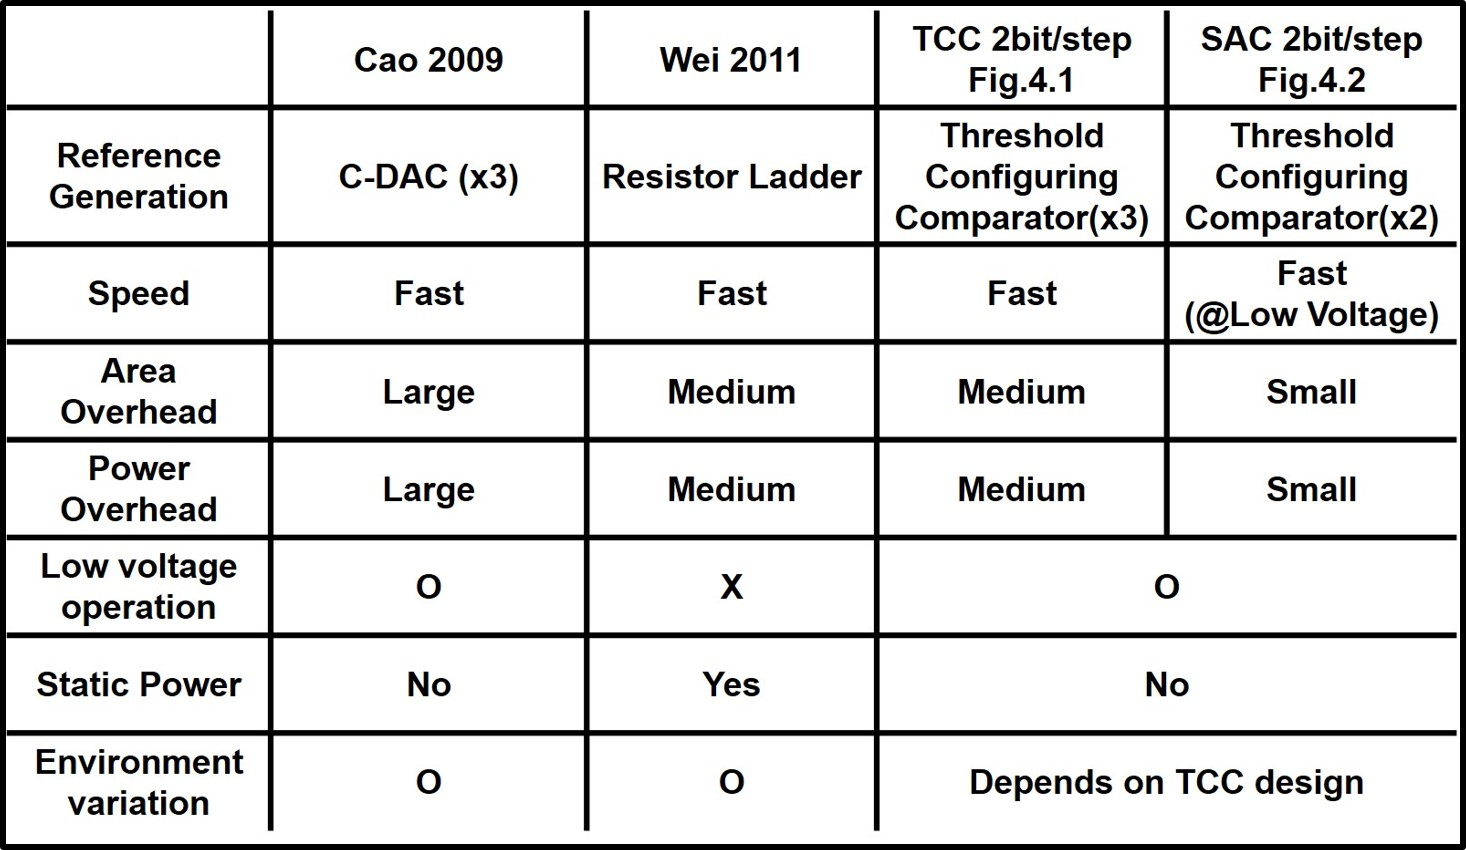
\includegraphics[width=0.9\textwidth]{figure/chap4/table1.jpg}
  \label{tab-4-1}
\end{table}

A 2-bit/step method uses a 2-bit quantizer inside the successive approximation (SA) loop to speed up the conversion. Because only $n$/2 cycles are required for the $n$ bit conversion, the SAR ADC speed can be ideally doubled. Since the SAR logic requires little modification to realize the 2-bit/step operation, there is a small overhead in the digital circuitry. However, providing a 2-bit quantizer requires many additional analog components and the ADC experiences a large power and area overhead. For example, Flash ADC is a preferred choice for the 2-bit quantizer. It can acquire the comparison results in one clock cycle but the reference of the Flash ADC must be configured every SA cycle. 

For example, at the 1st SA cycle, the references should be 1/4, 2/4, 3/4 $V_{ref}$, respectively. Before proceeding to the next cycle, the C-DAC switches its capacitors reflecting the comparison results. Therefore, references for the 2nd SA cycle must be 7/16, 8/16, 9/16 $V_{ref}$, respectively. Conventional 2-bit/step SAR ADC researches with a different generation of references are described in TABLE \ref{tab-4-1}. Previous researches require addition reference generation circuitry's (R-DAC and C-DACs) and consume an additional power overhead.
We try to minimize the overheads of the 2-bit/step operation by utilizing threshold configuring comparators.


\subsection{2-bit/step with threshold configuring comparators}

\begin{figure}
\centering
  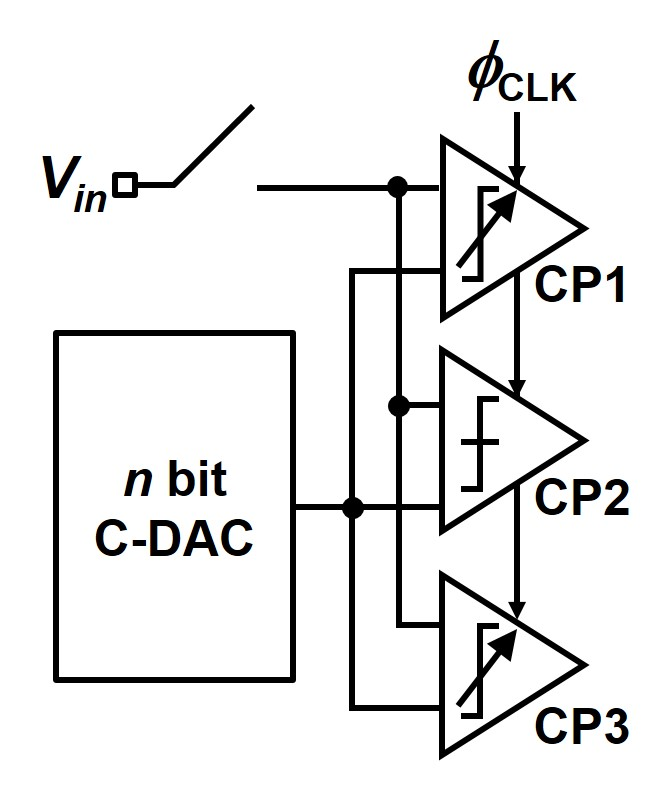
\includegraphics[width=0.6\textwidth]{figure/chap4/fig1.jpg}
  \caption{Block diagram of a 2-bit/step ADC provided with TCC.}
  \label{fig-4-1}
\end{figure}

Our key idea is: instead of using multiple references, we realize the 2-bit/step operation by configuring comparator offsets (or threshold $V_{offset}$). A simple block diagram of our proposed 2-bit/step SAR ADC implemented with a threshold configuring comparator (TCC) is shown in Fig. \ref{fig-4-1}. 

CP2 is an ordinary comparator, which simply compares the input signals $V_{in}$ and VDAC. Suppose that $V_{offset}$ of 1/4 $V_{ref}$ and -1/4 $V_{ref}$ are applied to comparator CP1 and CP3. The comparator threshold ($V_{THcomp}$) would be 3/4 $V_{ref}$ and 1/4 $V_{ref}$, respectively and 2-bit quantizer is provided. In this method, at a certain SA cycle $N$, $V_{offset}$ of CP1 and CP3 should be:
\begin{equation}
    V_{offset} = \pm \frac{1}{2^2N}
\end{equation}
When foreground calibration is done and $V_{offset}$ is set properly, our proposed method will require only one C-DAC and sampling switch respectively. Therefore, power can be significantly reduced when compared with \cite{cao200932} and ADC does not consume DC power. 

However, several power and area overheads remain in this TCC based 2-bit/step SAR ADC. First, because the comparators must configure their threshold each cycle, there is a dynamic power of $V_{offset}$ control circuit. Second and most critically, there is an overhead in comparator activation. While an ordinary SAR will require only 2 comparator activations in a 2-bit conversion, such a 2-bit Flash operation requires 3 comparators to be activated. As a result, comparator power increases by 50\%. The issue is more critical because TCC consumes more power than normal comparators.

\subsection{2-bit/step with Successively Activated Comparators}

\begin{figure}
\centering
  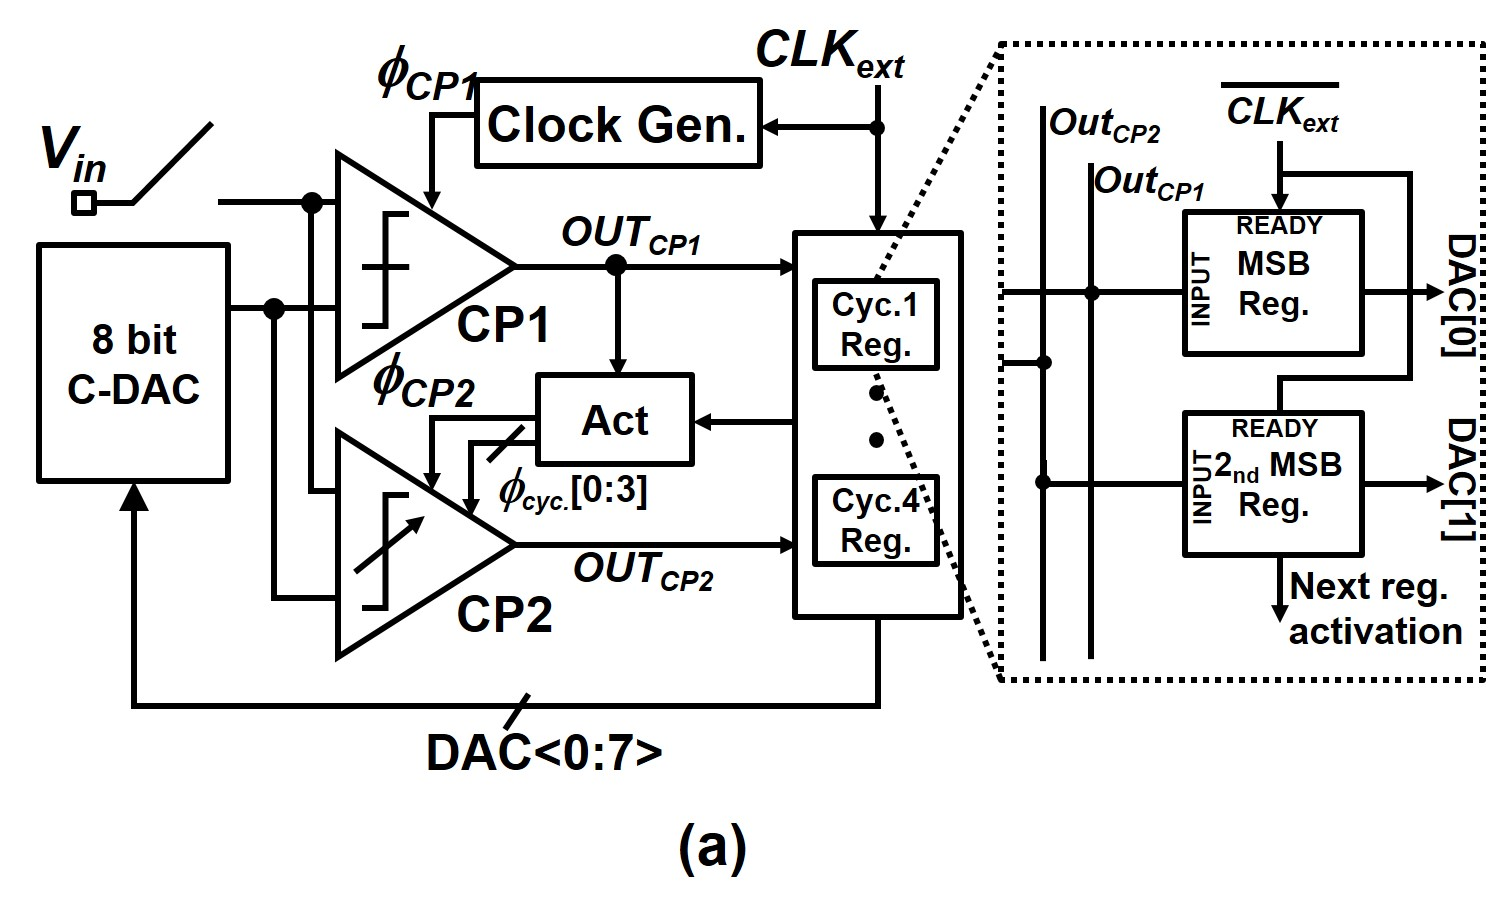
\includegraphics[width=0.9\textwidth]{figure/chap4/fig2a.jpg}
  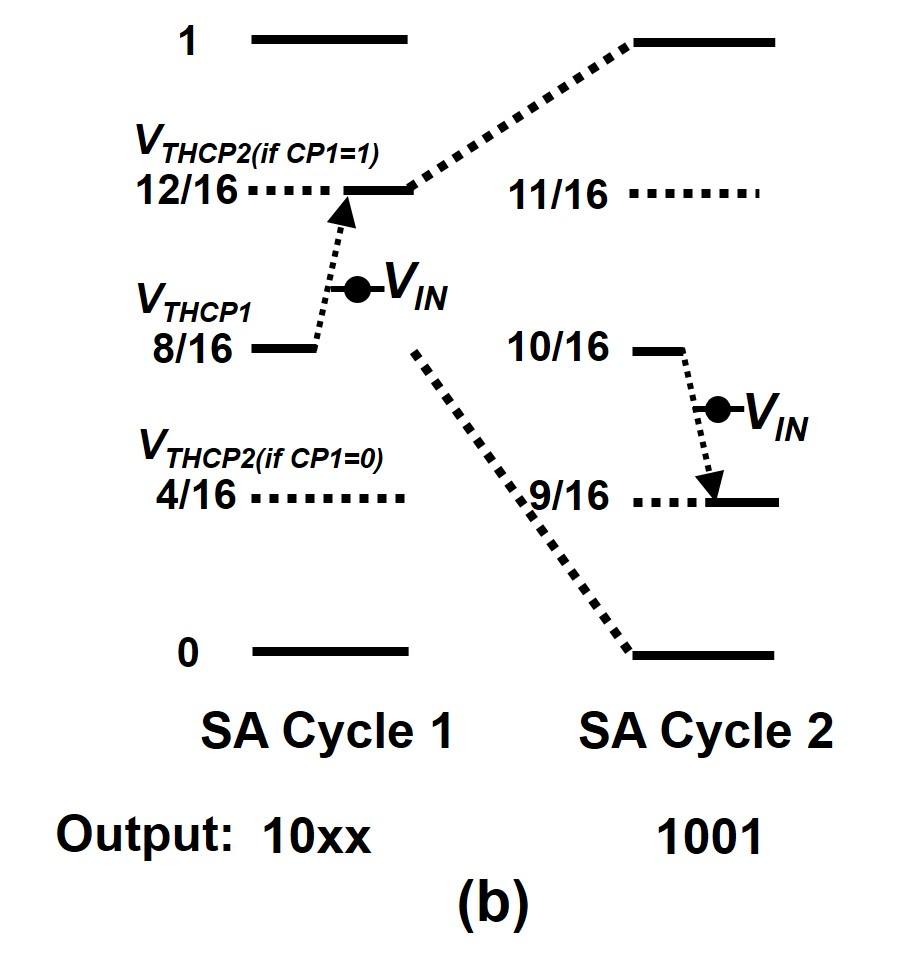
\includegraphics[width=0.7\textwidth]{figure/chap4/fig2b.jpg}
  \caption{Proposed 2-bit/step SAR ADC with successively activated comparators.    (a) Block diagram. (b) Operation concept.}
  \label{fig-4-2}
\end{figure}

For further power reduction, we propose a 2-bit/step ADC with successively activated comparators (SAC) and the block diagram and operation concept is shown in Fig. \ref{fig-4-2}. After the external sampling clock ($CLK_{ext}$) sets down, a SA cycle 1 starts by rising $\phi$1 and CP1 decide the first bit ($OUT_{CP1}$). After the first bit decision, $V_{THcomp}$ of CP2 ($V_{THCP2}$) is set reflecting the result of the first bit. In this case $OUT_{CP1}$ is 1, thus $V_{THCP2}$ is set to 12/16 $V_{ref}$ and the second bit ($OUT_{CP2}$) is decided. In the proposed ADC the 2-bit quantizer operates like a binary-search ADC \cite{van2008150}, where the second comparator is activated reflecting the preceding comparator’s results. Because the second comparator threshold is configured dynamically every cycle, only two comparators are required instead of three. 
The results of SA cycle 1 are stored in MSB and 2nd MSB registers respectively.

\begin{figure}
\centering
  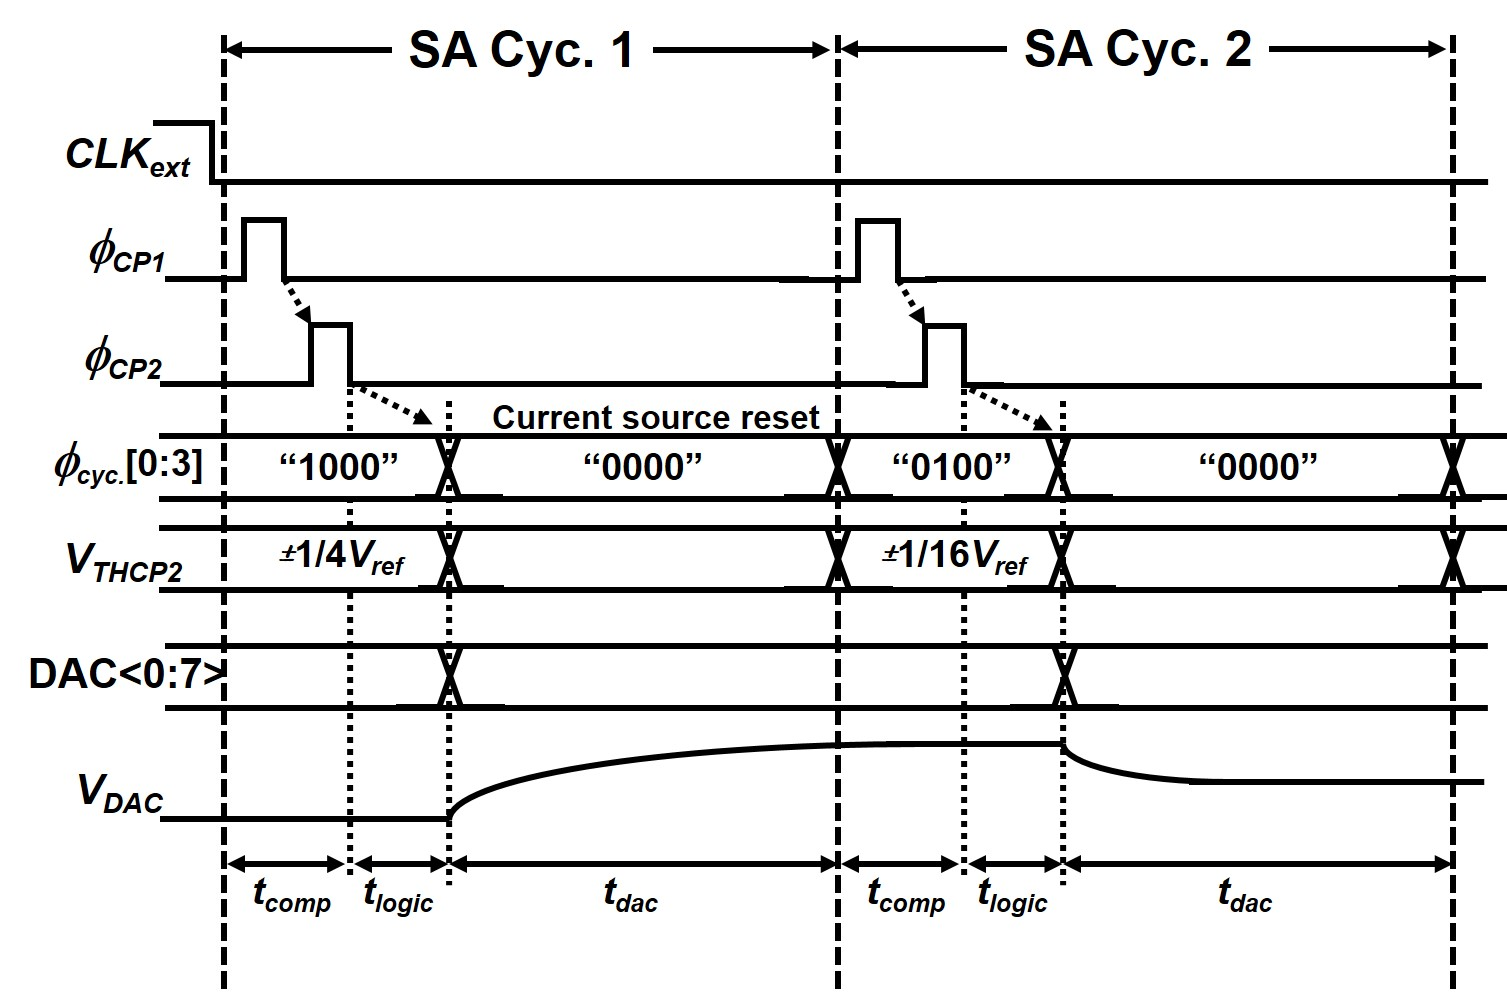
\includegraphics[width=0.9\textwidth]{figure/chap4/fig3.jpg}
  \caption{Timing chart of the proposed ADC.}
  \label{fig-4-3}
\end{figure}

Fig. \ref{fig-4-3} shows the timing chart of the proposed ADC of SA cycle 1 and 2. Here, CP1 is activated by $\phi$CP1 when the sampling signal($CLK_{ext}$) sets down, and then $\phi$CP2 rises successively and 2-bit output is acquired. After the register latches the comparator outputs, ADC cycle signal($\phi$cyc.) change and the ADC prepares for SA cycle 2. However, before the next comparison starts, a VDAC settling delay($t_{DAC}$) is inserted for the reference settling. $\phi$cyc.[0:3] is used to control $V_{THCP2}$, since it must be configured every cycle. After sufficient C-DAC settling, $\phi$CP1 rises and SA cycle 2 begins. By repeating these procedures, this ADC achieves an 8-bit conversion with 4 SA cycles.

A genetic SAR ADC cycle time is determined by three delays: comparator delay($t_{comp}$), SAR logic delay($t_{logic}$), and DAC settling($t_{DAC}$). Therefore, the total conversion time of an 8-bit 1-bit/step SAR ADC is assumed 8($t_{comp}$+$t_{logic}$+$t_{DAC}$). On the other hand, the conventional 2-bit/step SAR ADC conversion time is only 4($t_{comp}$+$t_{logic}$+$t_{DAC}$), since 2-bits are processed simultaneously. Next, our proposed circuit is considered. The timing chart in Fig.3 implies that $t_{logic}$ and $t_{DAC}$ is halved but because the comparators are activated successively, there is no improvement in $t_{comp}$. Therefore, the conversion time for 8-bit SAC operation is: 

\begin{equation}
    t_{conversion} = 8 \times t_{comp}+4(t_{logic}+t_{DAC})
\end{equation}

We can draw a conclusion that the improvement in SAC speed is larger when $t_{comp}$ is shorter than $t_{logic}$+$t_{DAC}$. In a typical mid-resolution SAR ADC operated with a standard supply voltage, all the delays are about the same length. However, in low-voltage SAR ADCs, it is known that $t_{logic}$ and $t_{DAC}$ may be much longer than $t_{comp}$ \cite{sekimoto201140nm}: the SAC architecture will benefit in such low-voltage settings. For standard voltage settings, one may choose the ordinary 2-bit/step architecture and simply utilize three TCCs to obtain sufficient speed improvements.

\begin{figure}
\centering
  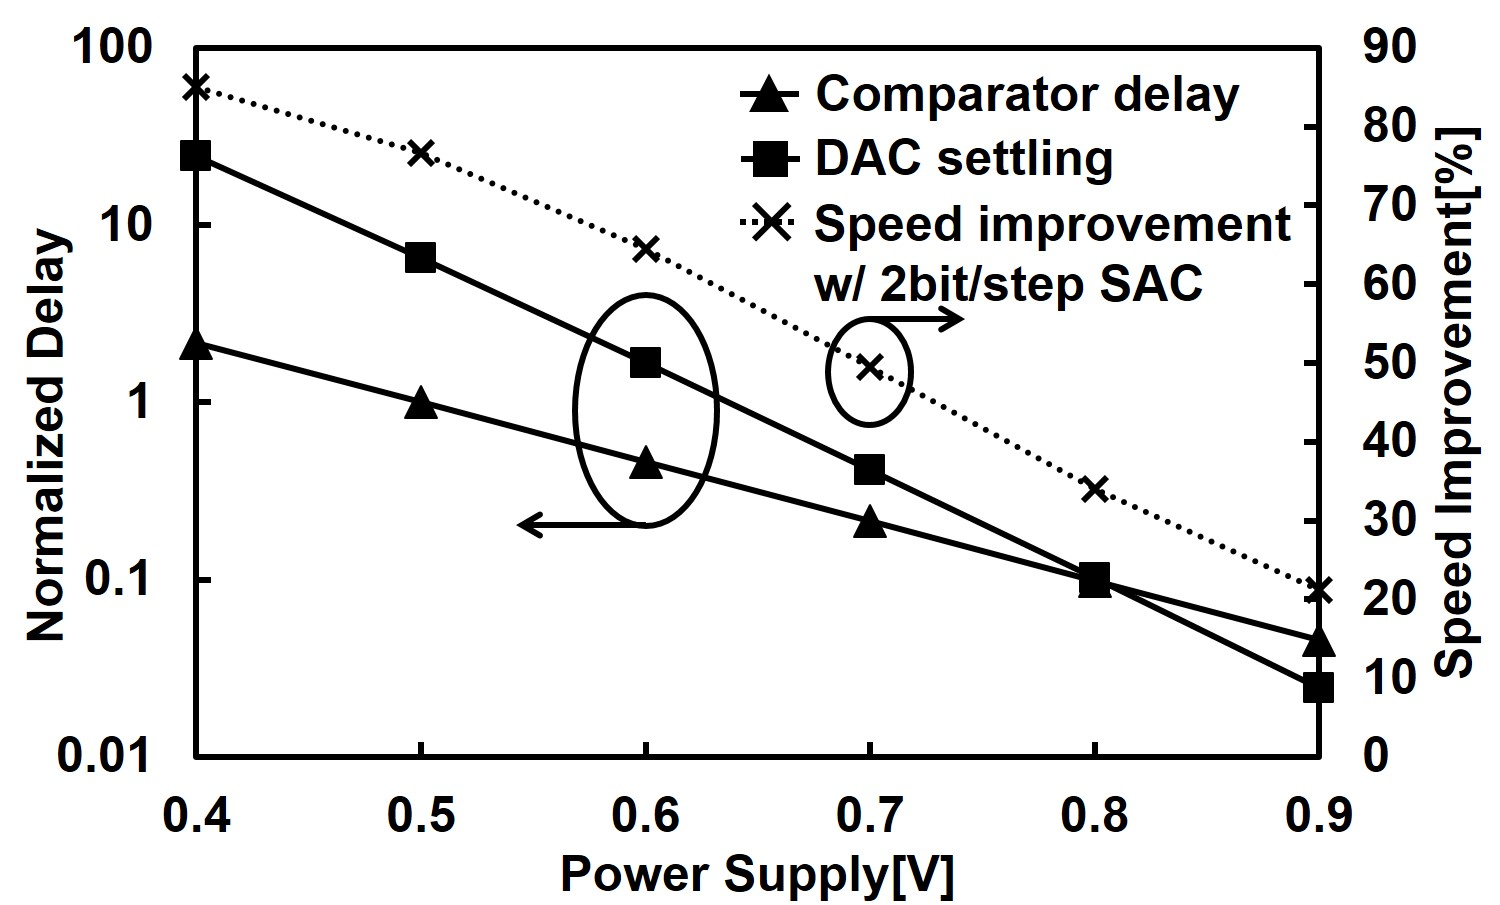
\includegraphics[width=0.9\textwidth]{figure/chap4/fig4.jpg}
  \caption{Power supply versus comparator delay, DAC settling and speed improvement respectively.}
  \label{fig-4-4}
\end{figure}

The power supply versus $t_{DAC}$ and $t_{comp}$ was obtained respectively using simulation results, plotted in Fig. \ref{fig-4-4} including speed improvement using SAC. At voltages lower than 0.6 V, the load capacitance determines the delay time and $t_{comp}$ is considerably shorter. Under such conditions, the proposed SAC significantly speeds up the ADC. However, as the power supply rises, drain current exponentially increases and the DAC buffer instantly charges large load capacitance. 
When the supply voltage exceeds 0.8 V, the overdrive voltage becomes the dominating constant and the ratio between $t_{comp}$ and $t_{DAC}$ flips. For such ADC designs, 2-bit/step ADC designs should use three TCCs to maximize the speed improvements.

\subsection{2-bit/step with a single threshold configuring comparator}
\begin{figure}
\centering
  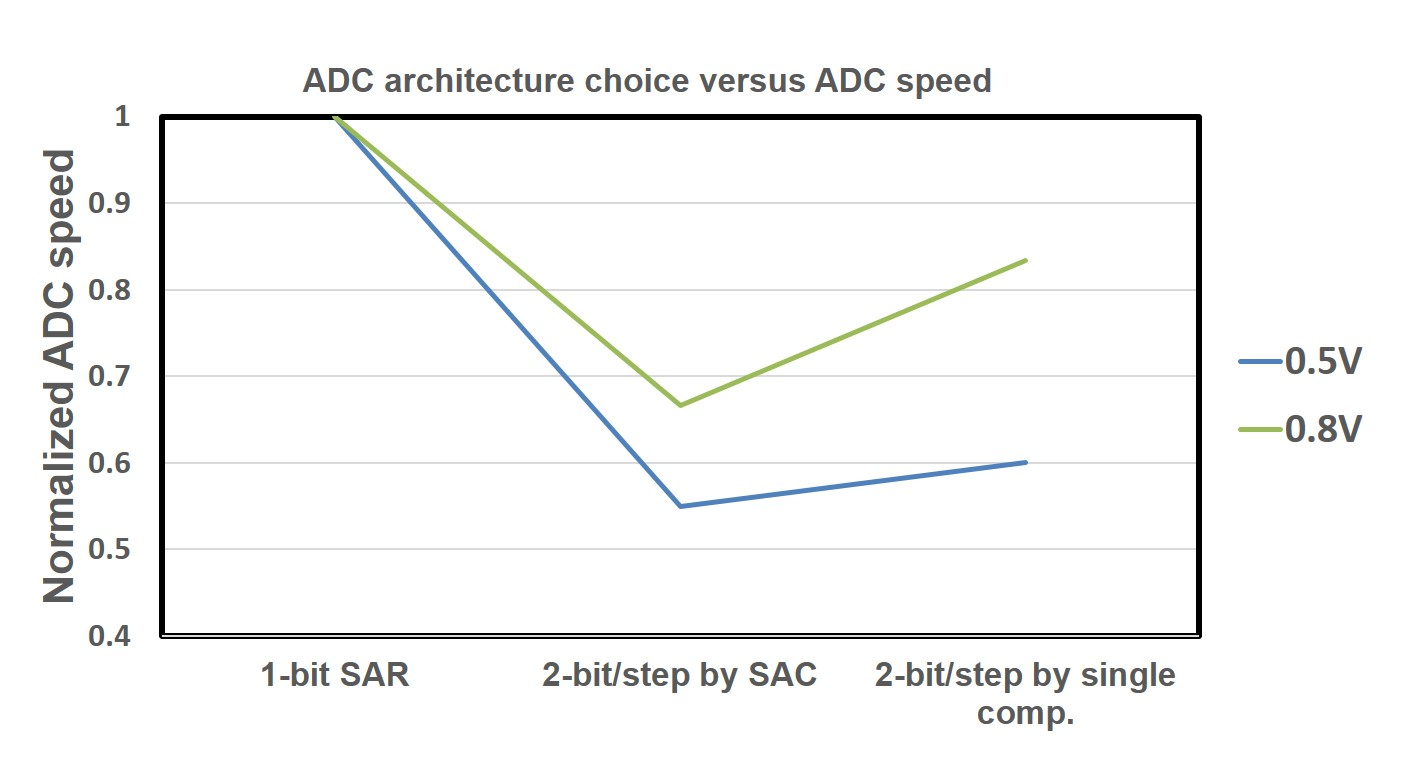
\includegraphics[width=1\textwidth]{figure/chap4/comp-vs-adc.jpg}
  \caption{ADC architecture choice versus ADC speed.}
  \label{fig-4-comp-vs}
\end{figure}
Notice that 2-bit/step operation can be done by a single comparator, by adding threshold configuring features to CP1 in Fig. \ref{fig-4-2} (a).
We will study the single comparator 2-bit/step operation and compare its performance versus the proposed SAC method.
First of all, since the operation can be concluded with a single comparator, the single comparator 2-bit/step can save 20\% of the circuit area. However, the 8-bit conversion time consists of:
\begin{equation}
    t_{conversion} = 8 \times t_{comp} + 4 \times t_{reset} + 4(t_{logic}+t_{DAC})
\end{equation}
While SAC does not include the comparator reset time ($t_{reset}$) in its critical path, the single comparator implementation additionally includes the reset time. 
Here, we will estimate that the reset time is similar to the comparison time.
While the single comparator can improve the conversion speed when the DAC settling time is dominant (at low voltage conditions), speed improvements are limited if DAC settling and comparator time are similar (standard voltage conditions). This is plotted in Fig. \ref{fig-4-comp-vs}, where at 0.5V, the SAC and single comparator settings achieve a similar speed improvement. However, at 0.8V, the speed improvements of single comparator settings become limited.
We can conclude that to achieve speed improvements at various supply voltage conditions, SAC architecture is more suited.

\section{Wide range threshold configuring comparator}

\begin{figure}
\centering
  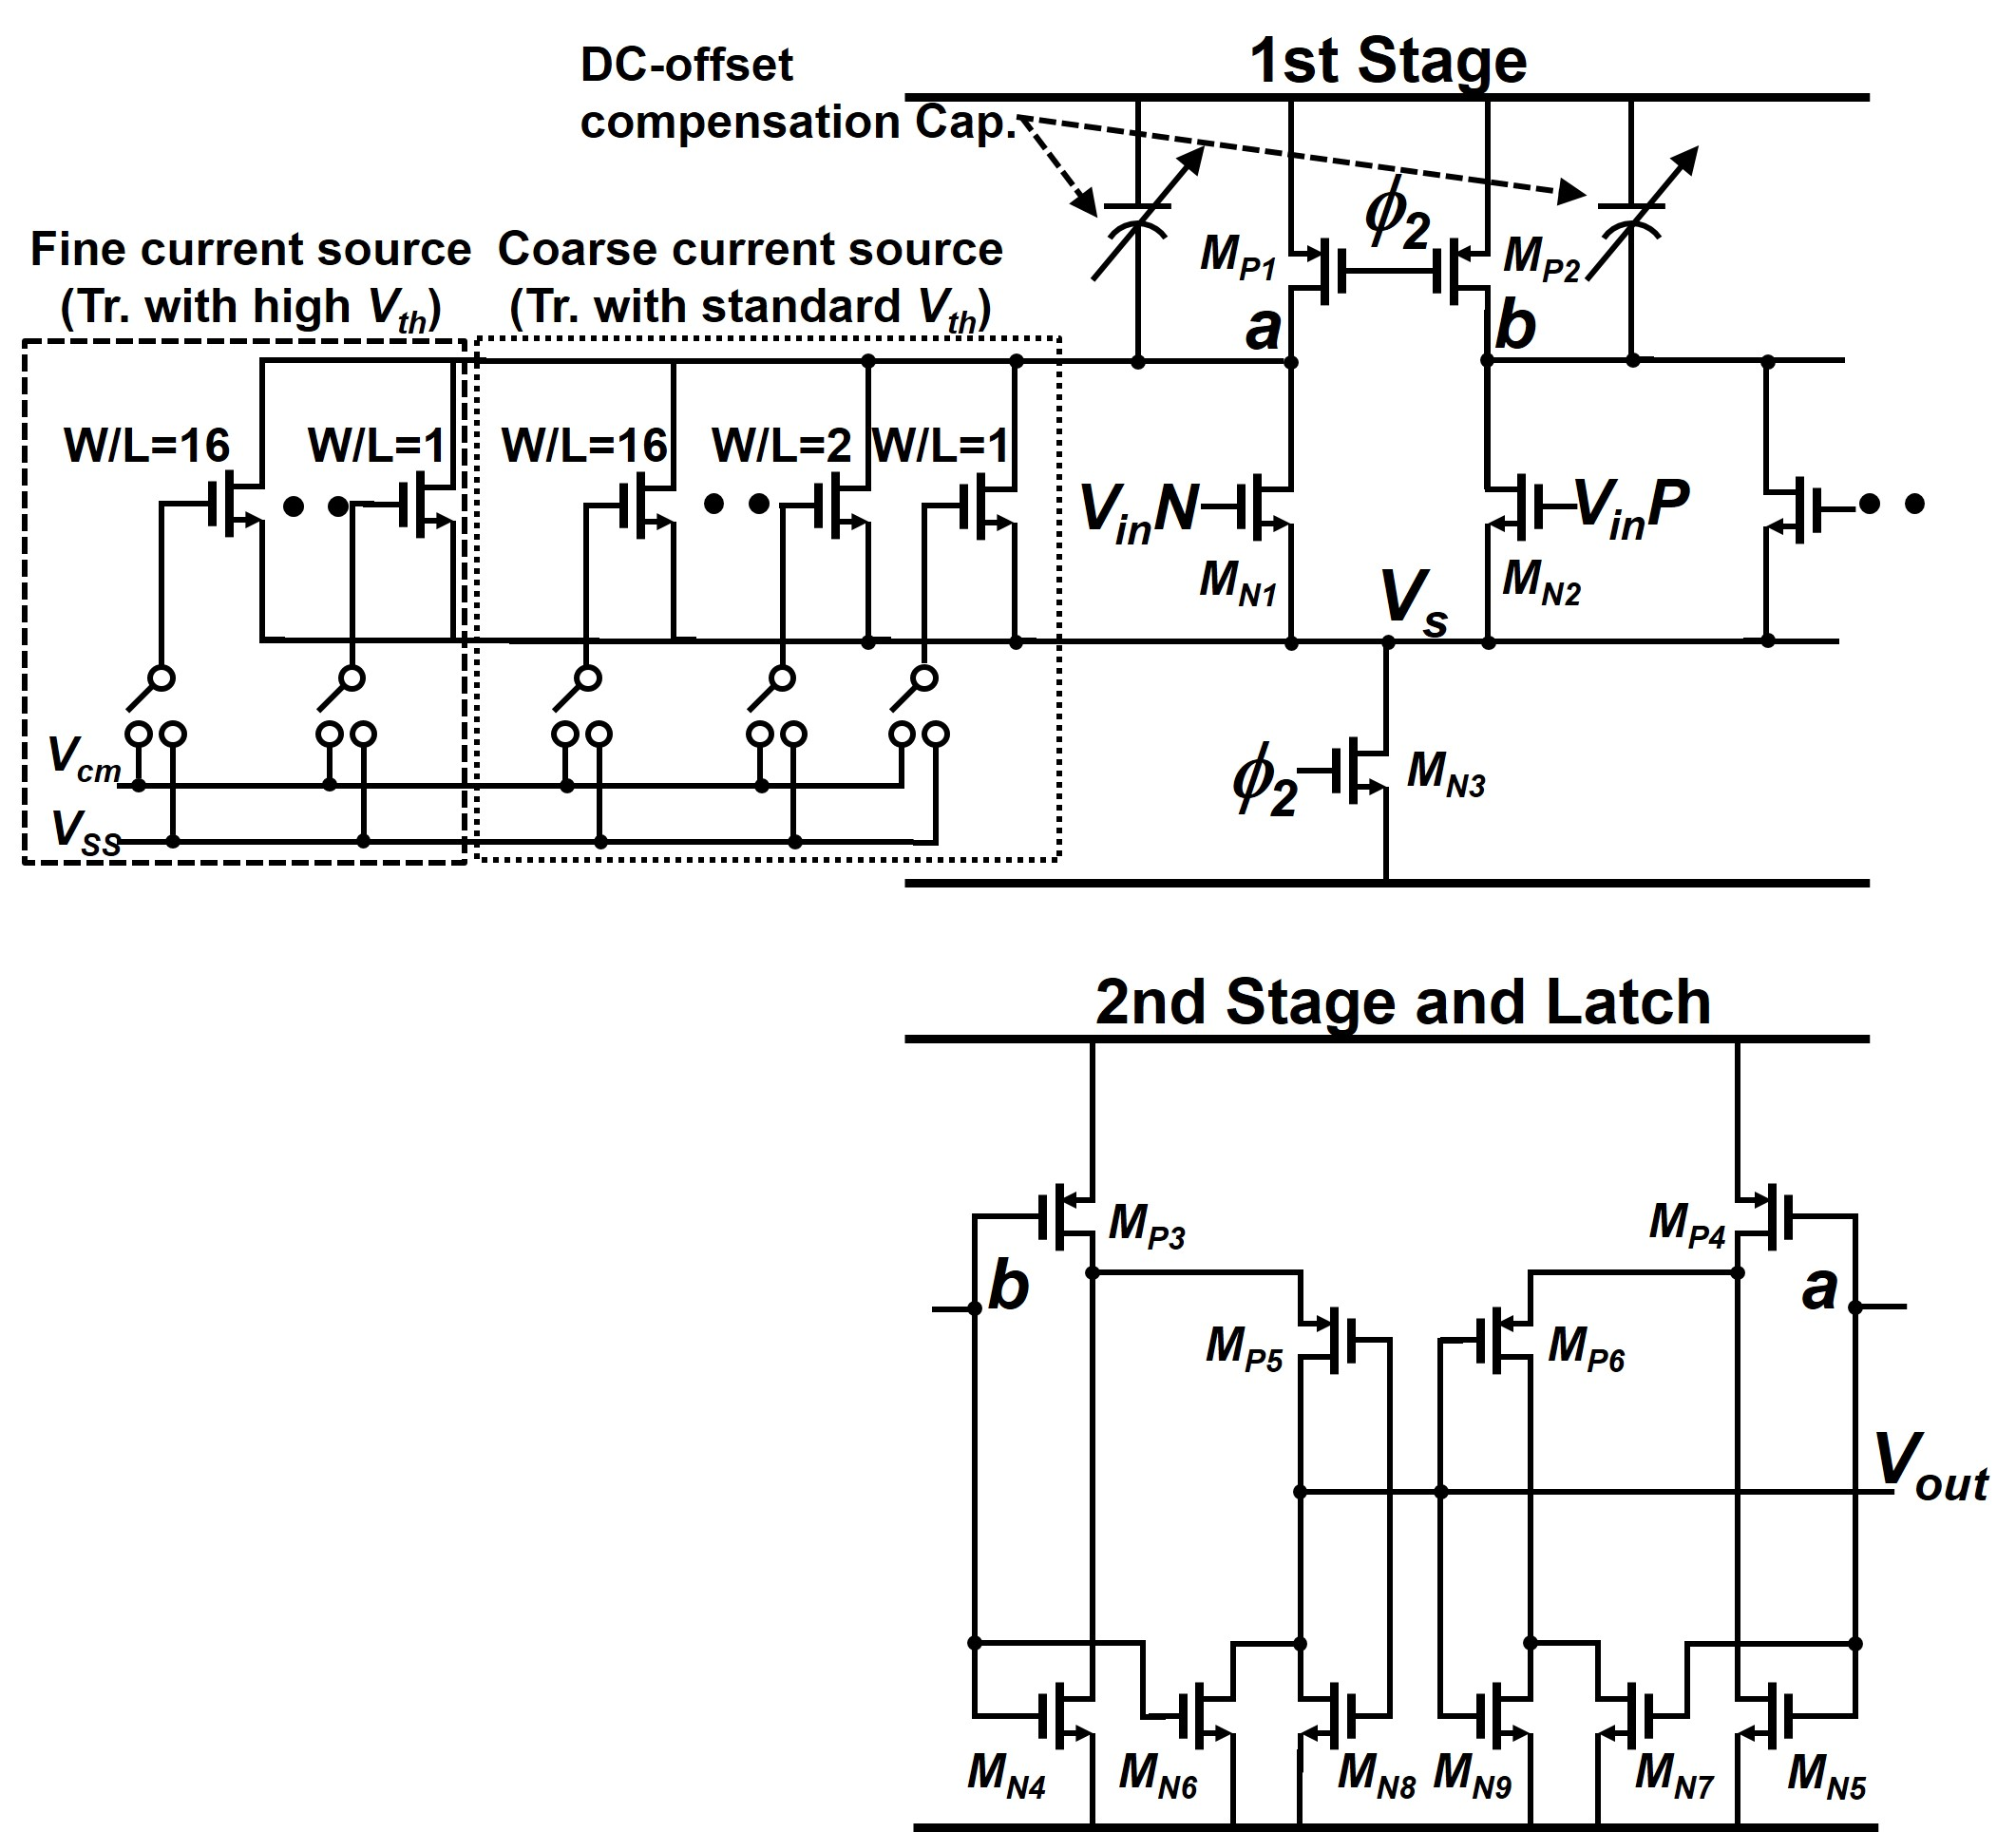
\includegraphics[width=1\textwidth]{figure/chap4/fig5.jpg}
  \caption{Threshold configuring comparator design.}
  \label{fig-4-5}
\end{figure}

\subsection{TCC Architecture}

To compensate for comparator offsets from process mismatches, TCCs have been widely used. 
A common TCC is provided by asymmetric capacitive loads \cite{nuzzo-thresholdconfiguring} \cite{verbruggen-dynamicpipeline} and also current sources are frequently used \cite{miyahara2008low} \cite{el-chammas-tcc}. Fig.\ref{fig-4-5} shows the comparator schematic with threshold configuring used in CP2. CP1 does not have the threshold configuring element but the basic architecture is the same. 

Our TCC architecture is based on a Miyahara two-stage dynamic comparator \cite{miyahara2008low}. To start with, the basic comparator operation is described.  The comparison begins when the comparator activation signal ($\phi$2) becomes HIGH. Nodes a and b (the drain node of the input transistors MN1 and MN2) drop with its speed proportional to the gate voltage of the input transistors. When either drops $V_{latch}$, the second stage latch operates and the output is decided.

%After TCC output is decided, $\phi$2 sets down to $LOW$. MP1, MP2 are turned on and the comparator enters the regeneration phase. Therefore, nodes a,b are charged to $V_{DD}$. On the other hand, tail transistor MN3 is turned off and the source voltage of the input transistors (VS) is left floated. As a result, the voltage of VS is decided by the inputs $V_{inP}$ and $V_{inN}$. This can be a serious matter for the TCC since the source voltage is undetermined and the characteristics of input transistor and current sources may change. However, the charge stored in VS is remarkably small compared with charge stored in nodes a and b. The post-layout simulation at 0.6 V show that when $\phi$2 rises and comparisons begin, the drop of VS is much faster than that of a,b. The charge stored in VS is drawn out in 20 ps whereas the charge in a,b takes 250 - 500 ps to drop to the voltage which the latch operates. These results show that voltage of VS before comparison does not affect the result of TCC.

Next, we will review several conventional threshold configuring methods and compare them with our proposed method. 
A certain cycle when $V_{THcomp}$ is to be $V_x$ is supposed. Under this condition, the TCC should be balanced when $V_{inP}$, $V_{inN}$ =$V_{CM} \pm V_x$. The drain current of input transistors $I_{dP}$ and $I_{dN}$ in this condition are calculated, and the time until the results are latched ($t_{latch}$) can also be estimated as well. If the input differential pairs simply draw out charge $Q = C \times V_{latch}$ stored in nodes a and b,
\begin{equation}
    t_{latch}=(C*V_{latch})/I_d
\end{equation}
Since $t_{latch}$ should be the same for the both input transistor pairs, 
\begin{equation}
\frac{I_{dP}}{I_{dN}} = \frac{C_N}{C_P}
\label{eq7}
\end{equation}
can be led where $C_n$ and $C_p$ are load capacitance of nodes a and b. 
\eqref{eq7} is a very important, since it imposes that the comparator threshold configuring can be achieved by: 1) providing a gap (or an offset) of load capacitance between $C_N$ and $C_P$ or 2) by providing an offset current to $I_{dP}$ or $I_{dN}$ or 3) providing a $gm$ offset between the input transistors. 
However, a very wide threshold shifting of 3/4$V_{Ref}$ and 1/4$V_{Ref}$ are required to realize a 2-bit/step operation in cycle 1 (Fig.\ref{fig-4-2}(b)) and this is challenging with offset load capacitance. To realize such $V_{THcomp}$, simulation results at 0.5V shows that an impractical capacitance of $\Delta$C = 7.7pF is required. Therefore, the comparator power will increase 5$\times$ and in addition, the comparison time will be significantly prolonged. This is because when realizing a large threshold shift at low supply voltages, the drain current of the two input transistors can differ as much as 100$\times$ when one enters sub-threshold region deeply and one does not. 

The same problem appears when implementing built-in comparator offset methods \cite{yoshioka-10b-50MS-SAR}, which create offset by asymmetrically tuning the tail currents (or can be realized by changing the $g_m$ of the input transistors). Tail current configuring will require sizing that is proportional to $I_{dP}/I_{dN}$ and at low voltages, transistor arrays with W/L sizing exceeding 100$\times$ will be required. This will significantly increase the comparator area.

In our proposed TCC, the $V_{THcomp}$ is widely configured by a variable current source (VCS). For example, when the $V_{THcomp}$ is set to 12/16 $V_{Ref}$, the VCS connected to the drain of $V_{inN}$ input transistor (node a) is activated. An offset current (IVCS) is added to $I_{dN}$ in \eqref{eq7} to match $I_{dp}=I_{dn}+I_{VCS}$. On the other hand, to set $V_{THcomp}$ to 4/16$V_{Ref}$, VCS connected to the drain of $V_{inP}$ input transistor are activated(node b). Note that the offset current configures $V_{THcomp}$ and capacitor loads are unchanged. Therefore, $t_{comp}$ is not prolonged in this design. 

However, by using the current sources, the overall current is increased and power consumption may increase as well. This can be neglected by operating the comparator dynamically; the transistors MP1 and MP2 are kept off during operation. Therefore, the overall charge drawn out at a single comparison does not change and the increase in comparator power is small. However by adding VCS, the parasitic capacitance at nodes a and b increases which increases the comparator power consumption by 15\%.

\subsection{TCC by variable current source}

Designing a bias circuit for VCS under various voltage conditions, including extremely low voltages, are very challenging. A bias circuit such as band-gap reference has resistance against temperature variation but cannot be used at low-voltages. Therefore, a simple biasing technique is required. A simple way is to use $V_{DD}$ as the bias voltage for the current sources. However, such a current source has a critical weakness against power supply noise. 

To improve the immunity to power supply noise, we propose the $V_{CM}$ biased VCS. Upon implementation, $V_{CM}$ biased NMOS transistors with binary tuned W/L ratios are used, as in Fig. \ref{fig-4-5}. Two types of transistor threshold, standard $V_{th}$ and high $V_{th}$ devices were used for ‘coarse’ and ‘fine’ VCS, configurable for 4 and 5-bit respectively. The use of different $V_{th}$ relaxes the transistor sizing greatly since the W/L ratio does not increase exponentially. Although the transistor $V_{th}$ and sizing differs between the coarse and fine VCS, the same operation and design methodology discussed below is adapted.

\begin{figure}
\centering
  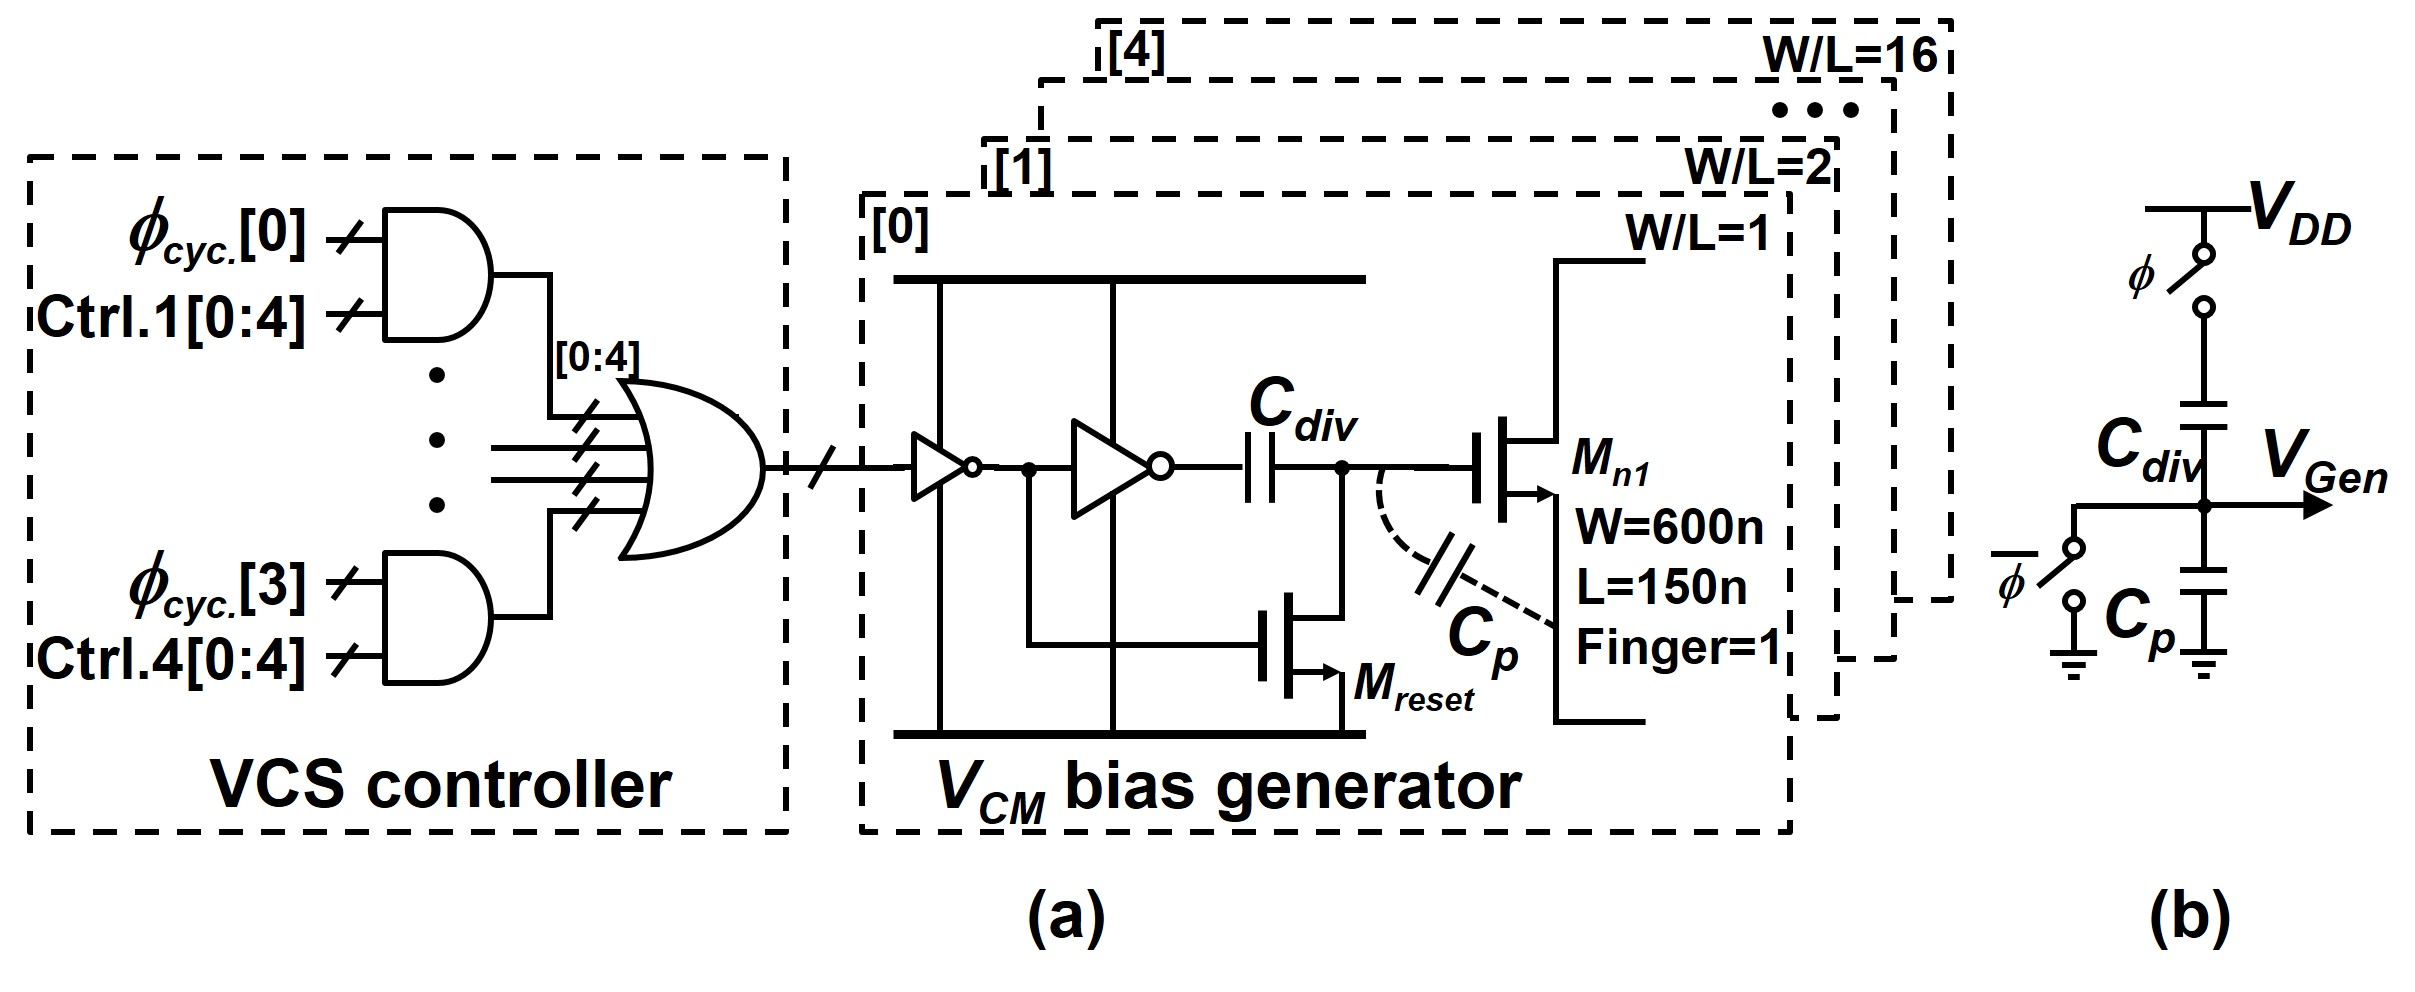
\includegraphics[width=0.9\textwidth]{figure/chap4/fig6.jpg}
  \caption{(a) Schematic of 5-bit Vcm biased variable current source.
(b) Operation of capacitive dividing.}
  \label{fig-4-6}
\end{figure}

Fig. \ref{fig-4-6}(a) shows the specific schematic of 5-bit $V_{CM}$ bias generation circuit and the control circuit of VCS. Here, Ctrl.1[0:4] to Ctrl.4[0:4] are values earned from calibration which determines VCS output for cycle 1 to 4 respectively. The Ctrl. signals are selected by the $\phi$cyc. signal(Fig. \ref{fig-4-3}), which rise at a specific cycle. The current source operates when the input of the bias generator is High. By capacitive dividing, a gate voltage of $V_{CM}$ is generated as shown in Fig.\ref{fig-4-6}(b). The capacitance value of $C_{div}$ is designed to be the same as the gate capacitance of the biased transistor MN1 and parasitic summed ($C_p$). In this design, $C_{div}$ was constructed by the MOM capacitor and its capacitance was designed to match the estimated $C_p$. Therefore, when the top plate of $C_{div}$ is connected to $V_{DD}$, capacitive dividing provides a gate voltage of $V_{Gen}=V_{CM}$. To eliminate hysteresis effects, the gate voltage must be reset after each comparison. During the DAC settling phase, $\phi_{cyc}$. is turned to Low which activates transistor Mreset in all VCS. By Mreset, the gate voltage of MN1 is reset to ground.

While $V_{CM}$ voltage is typically supplied on-chip, one can simply directly use this voltage as reference. 
However, CMOS switches to bypass $V_{CM}$ with high-speeds were difficult to design with low-voltages and fast transitions were not available. Since our target is realizing a fast 2-bit/step SAR ADC, such speed overheads were not acceptable.
Therefore, we chose an option to internally generate $V_{CM}$ like voltages at the comparator level. The voltages to charge the capacitors are $V_{DD}$ so the switching is very fast and does not corrupt the ADC conversion speeds.

\subsection{Variable current source design}

The specific design methods of the VCS are explained. The key points when designing VCS is deciding fundamental W and L sizing, implementation of $C_{div}$, and comparator noise increase. However, the W and L sizing is heavily dependent on process mismatch characteristics and should be decided based on the Monte-Carlo results.

In our design, the LSB current source transistor has a sizing of W = 600nm, L = 150nm with Finger = 1. For the larger bit, the Finger is increased by a multiple of 2 respectively. The LSB current source is sized so that it will configure $V_{THcomp}$ by 0.25 LSB(or 1/1024 $V_{Ref}$) and the mismatch is sufficiently small. Considering the process variation, this design margin is enough to generate $V_{THcomp}$ required for SAC operation with an accuracy of 0.5 LSB.

\begin{figure}
\centering
  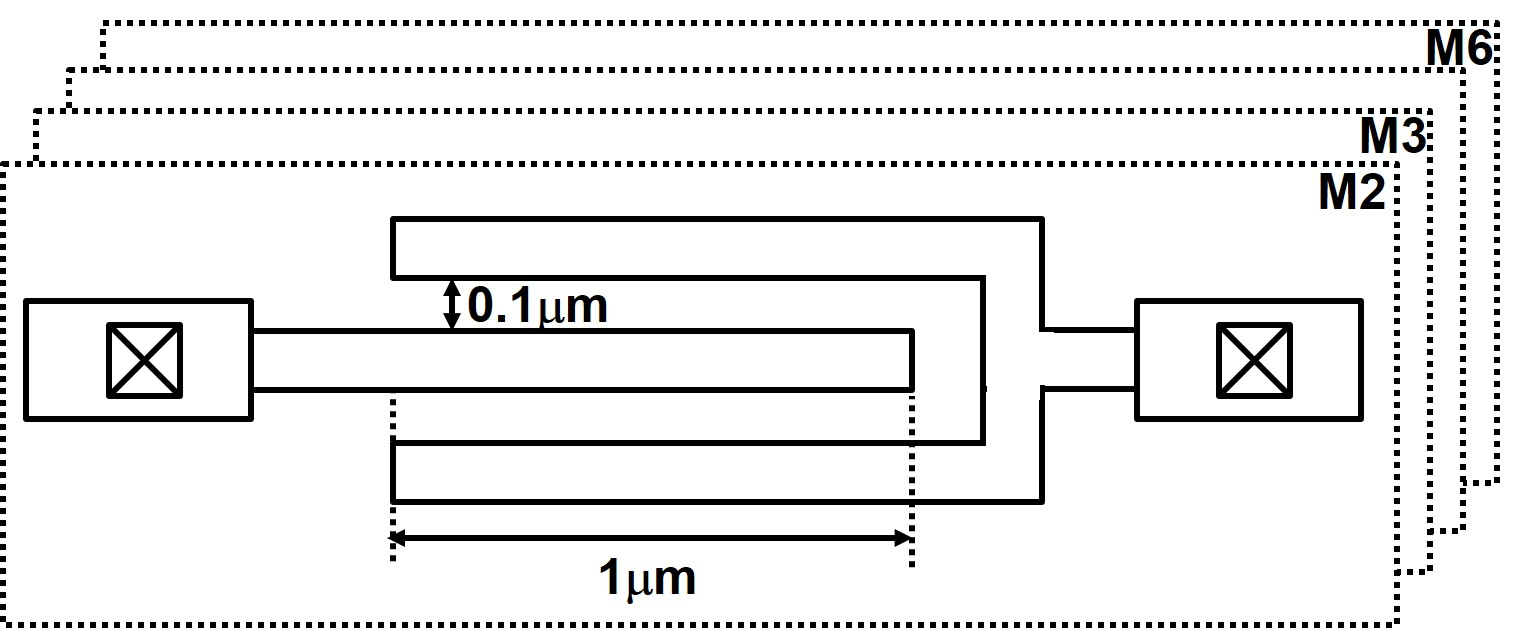
\includegraphics[width=0.9\textwidth]{figure/chap4/fig7.jpg}
  \caption{Area efficient 1 fF fringed capacitor used to provide $C_{div}$.}
  \label{fig-4-7}
\end{figure}

After fundamental values for W and L are decided, $C_{div}$ is calculated and implemented. We will suppose that a $V_{CM}$ bias circuit is designed for a transistor sizing of W = 600 nm, L = 150 nm, Finger = 8. A large L size was utilized to realize higher mismatch tolerance. The gate capacitance can be predicted from Cox, which is a portion of $t_{ox}$. For an example, if $t_{ox}$ = 25\AA, $C_{ox}$ will be 13.8fF/$um^2$. Therefore, $C_p$ can be roughly calculated: $C_p$ = $WLC_{ox}$ = 10fF. $C_{div}$ is created by a multi-layer fringed capacitor, which has high area efficiency. The capacitor occupies M2-M6 and Fig. \ref{fig-4-7} shows the capacitor of 1fF, which is used as a unit capacitor. Multi-layer fringed capacitors are challenging to be used in circuits which require precise matching, such as C-DACs, but are efficient for loose circuits. When designing $C_{div}$, one can run RC extraction to confirm that the calculation was right. 

A post-layout simulation run with the conditions above showed that 257 mV bias voltage is generated. However, $C_p$ relies heavily on W, L variation and operating region of the transistor as well. As a result, the capacitance can vary over 10\% than simulation results and makes accurate extractions meaningless. In this design, VCS does not require an accurate voltage of $V_{CM}$ to be generated and even though it varies, the ADC will still have power supply noise immunity. This issue is discussed specifically later on.

We also simulated the noise performance of the TCC as well. Since VCS injects additional noise to the comparator (and is not signal driven), the noise performance will degrade compared to normal comparators. While the CP1 comparator without VCS had an input-referred noise was 0.15 LSB, the TCC noise performance was 0.25 LSB, which increased the noise to 66\%. This is the worst condition, with all of the coarse current sources turned on. Still, the noise performance satisfies the ADC requirements in our design.
Generally, for TCCs, the input transistor $g_m$ has tougher requirements than ordinary comparators in which to cancel the noise generated by the VCS. This will not happen in capacitor load based TCCs \cite{nuzzo-thresholdconfiguring}, because bandwidth limitations of the capacitor load will improve the comparator noise performance.

\subsection{Power Supply Noise Immunity}

\begin{figure}
\centering
  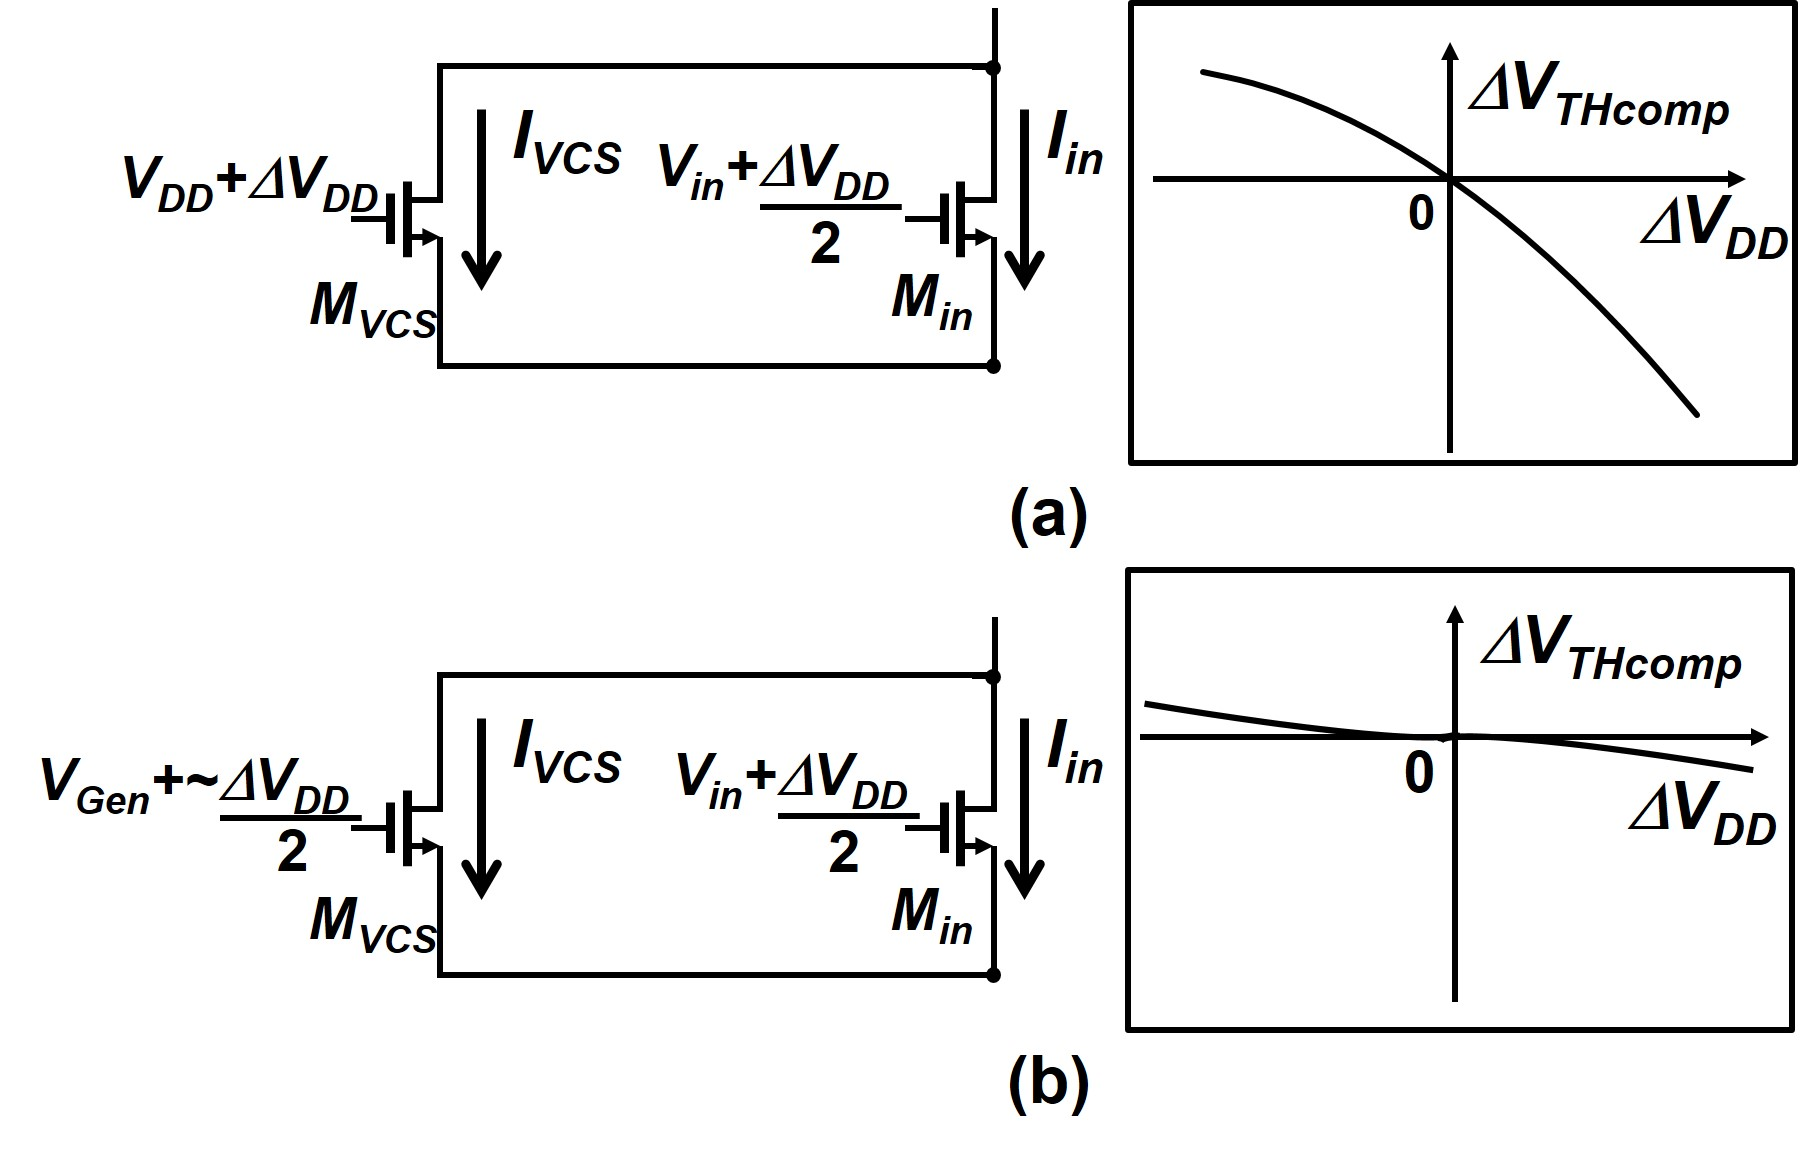
\includegraphics[width=0.9\textwidth]{figure/chap4/fig8.jpg}
  \caption{Power supply variation effect of 
(a)$V_{DD}$ biased VCS,  (b) $V_{CM}$ biased VCS}
  \label{fig-4-8}
\end{figure}

First, the power supply variation effect of the simple $V_{DD}$ biased current source will be studied as shown in Fig. \ref{fig-4-8}(a). We will suppose that the ADC input common-mode voltage is generated by dividing the ADC power supply voltage ($V_{DD}$) by half. Therefore, when there is a power supply voltage variation of $\Delta V_{DD}$, the ADC input($V_{in}$) varies $\Delta V_{DD}$/2. As a result, the gate-source voltage variation of the comparator input transistor is $\Delta V_{gsin}=\Delta V_{DD}$/2 but the variation of VCS transistor is $\Delta V_{gsVCS}=\Delta V_{DD}$. 
To summarize, in the case of $V_{DD}$ biasing, the effect of power supply variation is different between the input transistor which is a problem: the gate-source voltage difference between the VCS and input transistors will become an exponential difference in the current domain. 

For $V_{DD}$ biased current sources, even with a 10\% power supply drift, the TCC threshold will significantly drift and the ADC effective resolution will be around only 4 bits! 
Therefore, we must design the VCS current source so that the gate-source voltage difference between the VCS and input transistors will not occur when supply voltage changes.

The power supply variation effect with VCS biased by $V_{CM}$ is shown in Fig. \ref{fig-4-8}(b). When $V_{CM}$ bias generating circuit of Fig. \ref{fig-4-6}(b) is used, $V_{CM}$-like bias voltage $V_{Gen}$ is generated by capacitive dividing.
\begin{equation}
    V_{Gen} = \frac{C_{Div}}{(C_{div}+C_p) \times V_{DD}}
\end{equation}

If there were no mismatches, $C_{div}$/($C_{div}$+$C_p$)=0.5 will be realized and bias voltage of $V_{DD}$/2 will be generated. When the power supply voltage varies to $V_{DD}$+$\Delta V_{DD}$, the generated bias voltage will be affected as:
\begin{equation}
    V_{Gen2} = \frac{C_{Div}}{(C_{div}+C_p) \times (V_{DD}+\Delta V_{DD})}
\end{equation}
Hence, the gate-source voltage variation of the input transistors and the VCS transistors will be equal in the ideal case; the ADC gains tolerability against power supply variation. ($V_{Gen2}$=$V_{DD}$/2+$\Delta V_{DD}$/2 and $\Delta V_{gs}$ of $M_{in}$ and $M_{VCS}$, respectively will both be $\Delta V_{DD}$/2.)  
However, we need to consider non-ideal effects affected by process mismatch of $C_{div}$ and $C_p$. When power supply voltage varies to $V_{DD}$+$\Delta V_{DD}$ and there are mismatch in the two capacitor values, 
\begin{equation}
    | \Delta V_{gsVCS} - \Delta V_{gsin} | = \Delta V_{DD} \times |(C_{div}+C_p) - 0.5 |
    \label{eq17}
\end{equation}
Equation \eqref{eq17} implies that the more $C_{div}$/($C_{div}$+$C_p$) is closer to ideal (or 0.5), the TCC will cancel supply variation effects and ADC will hold more power supply variation resistance. 

\begin{figure}
\centering
  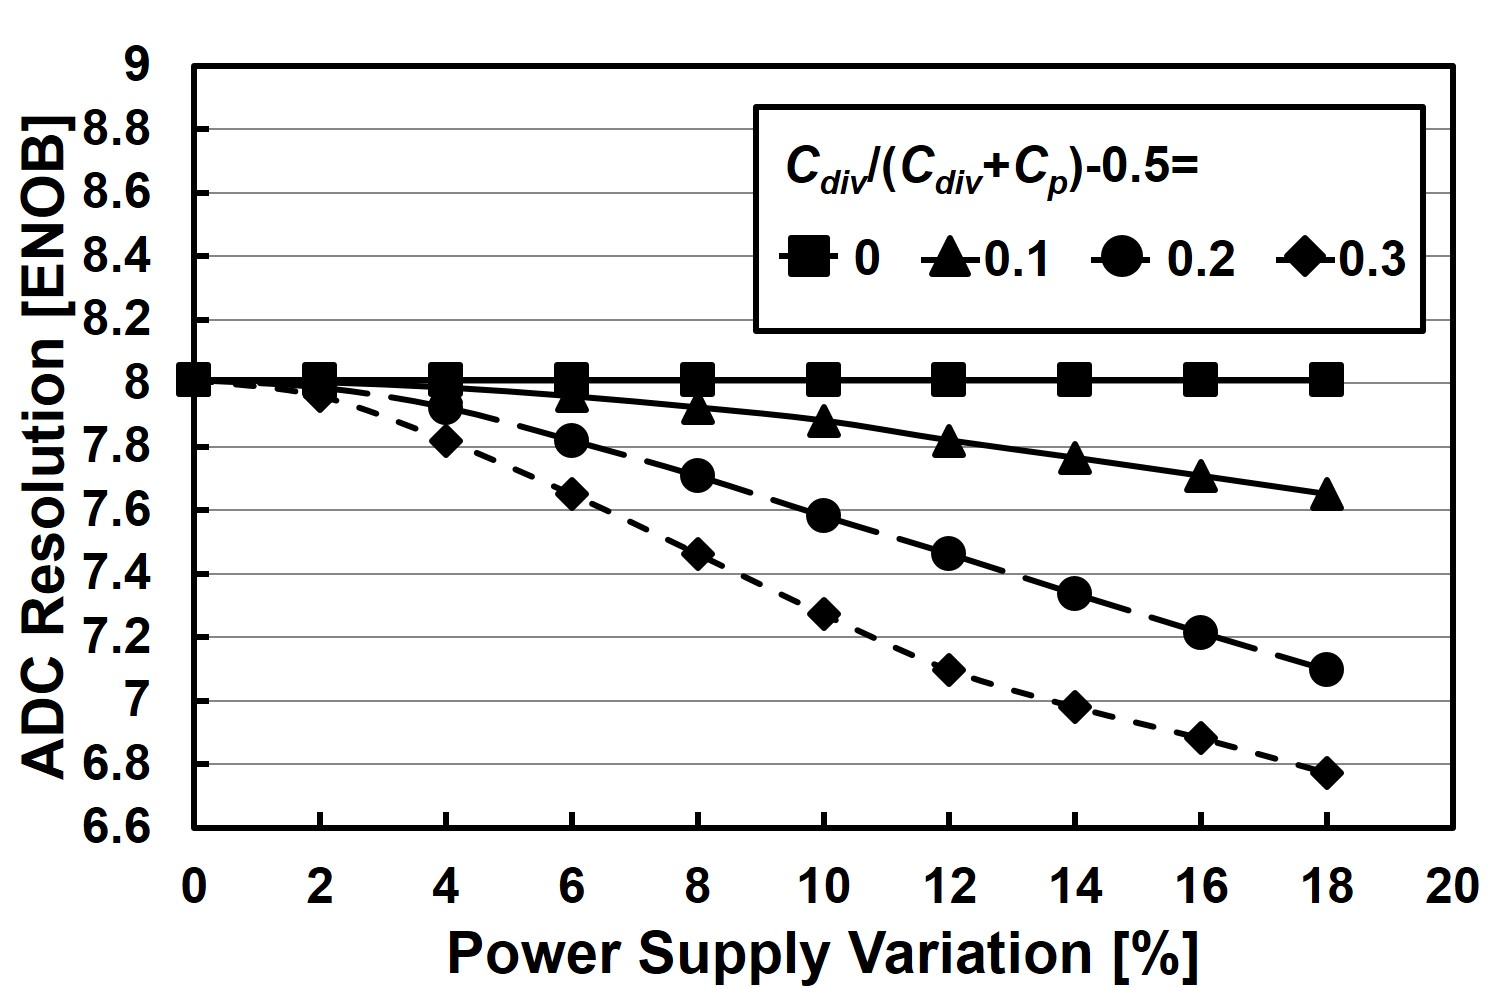
\includegraphics[width=0.9\textwidth]{figure/chap4/fig9.jpg}
  \caption{Power supply variation versus ADC resolution with different settings.}
  \label{fig-4-9}
\end{figure}

Fig. \ref{fig-4-9} shows the simulated results by Matlab which plots power supply variation versus ADC resolution in several mismatch conditions (modeled by $C_{div}$/($C_{div}$+$C_p$)-0.5). The supposed calibrated power supply is 0.5V. To maximize simulation efficiency, TCC (or CP2) including the VCS were modeled in Matlab, confirming consistency carefully with the simulation results. 
The rest of the 2-bit/step SAC ADC was modeled as well to obtain the resolution, where CP1 and DAC were assumed to be ideal. 
If ($C_{div}$/($C_{div}$+$C_p$)-0.5) is under 0.3 (meaning 20\% mismatch of ideal $V_{cm}$ and $V_{Gen}$), which can be sufficiently achieved even in 40 nm process, the ADC will achieve 7bit resolution with power supply variation of 10\%.

\subsection{Temperature variation effects}
Finally, temperature variation effects are discussed. The temperature effect can affect the transistor drain current in two ways, 1)change in mobility and 2)change in transistor $V_{th}$. Both mobility and $V_{th}$ has a negative temperature coefficient. 
However, while the decrease of mobility degrades $I_d$ as well, the $V_{th}$ decrease will increase $I_d$ exponentially. Since these effects contradict, $I_d$ calculation will be complex; when the $V_{gs}$ is small, the mobility change will be the dominating $I_d$ change and vice versa. Thus, depending on the comparator's input voltage, the offset drift due to temperature drift will be different. For example when the set threshold is large (e.g. 1st SA cycle), the set threshold voltage will drift largely from the calibrated value and for later SA cycles, the effect will be smaller. We conducted a temperature varying simulation based on the settings of Fig.\ref{fig-4-9}. Note that the simulated results are shown along with the measured results (in Fig.\ref{fig-4-17}).
At 400 K, there can be a 2-bit resolution decrease in the ADC. This is a serious issue if the ADC is operating in an environment where large temperature variation is expected. However, the effect should be countered by running $V_{THcomp}$ calibration periodically.


\section{Measurement Results}

\begin{figure}
\centering
  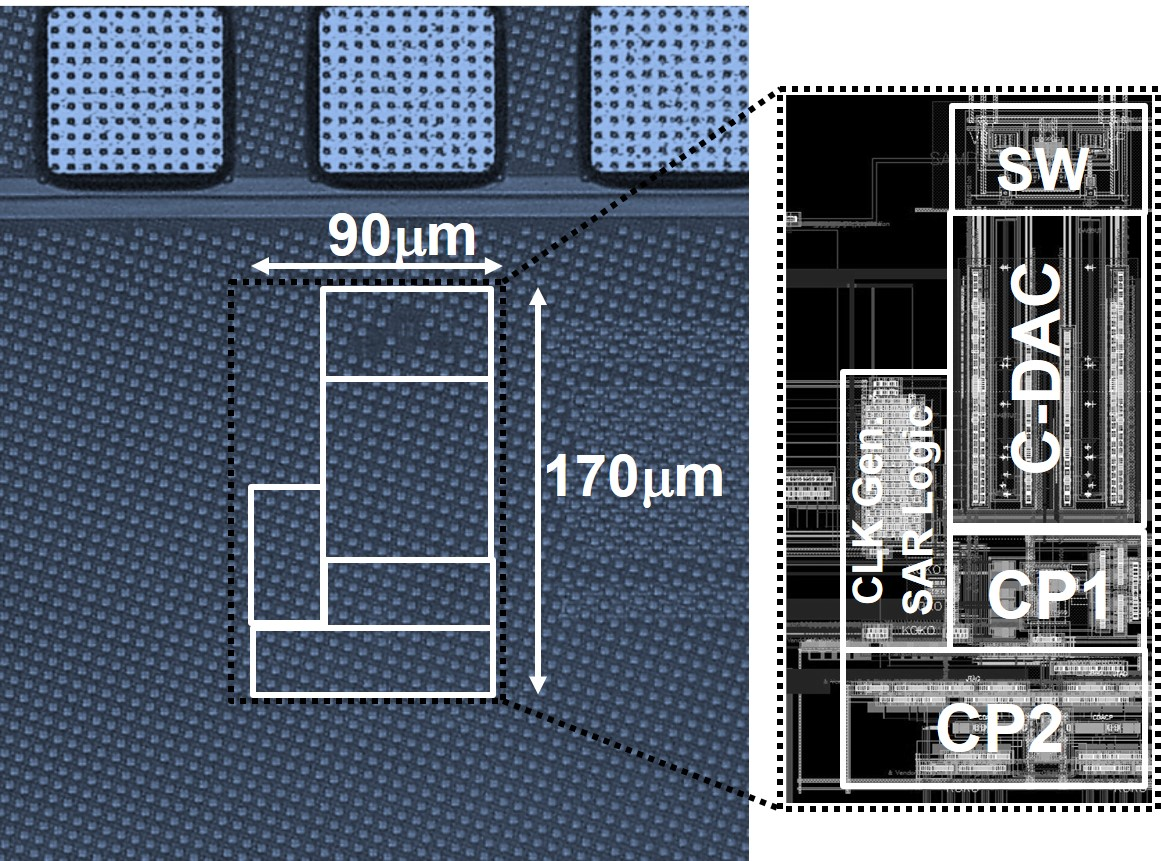
\includegraphics[width=0.7\textwidth]{figure/chap4/fig10.jpg}
  \caption{Chip photo.}
  \label{fig-4-10}
\end{figure}

\begin{figure}
\centering
  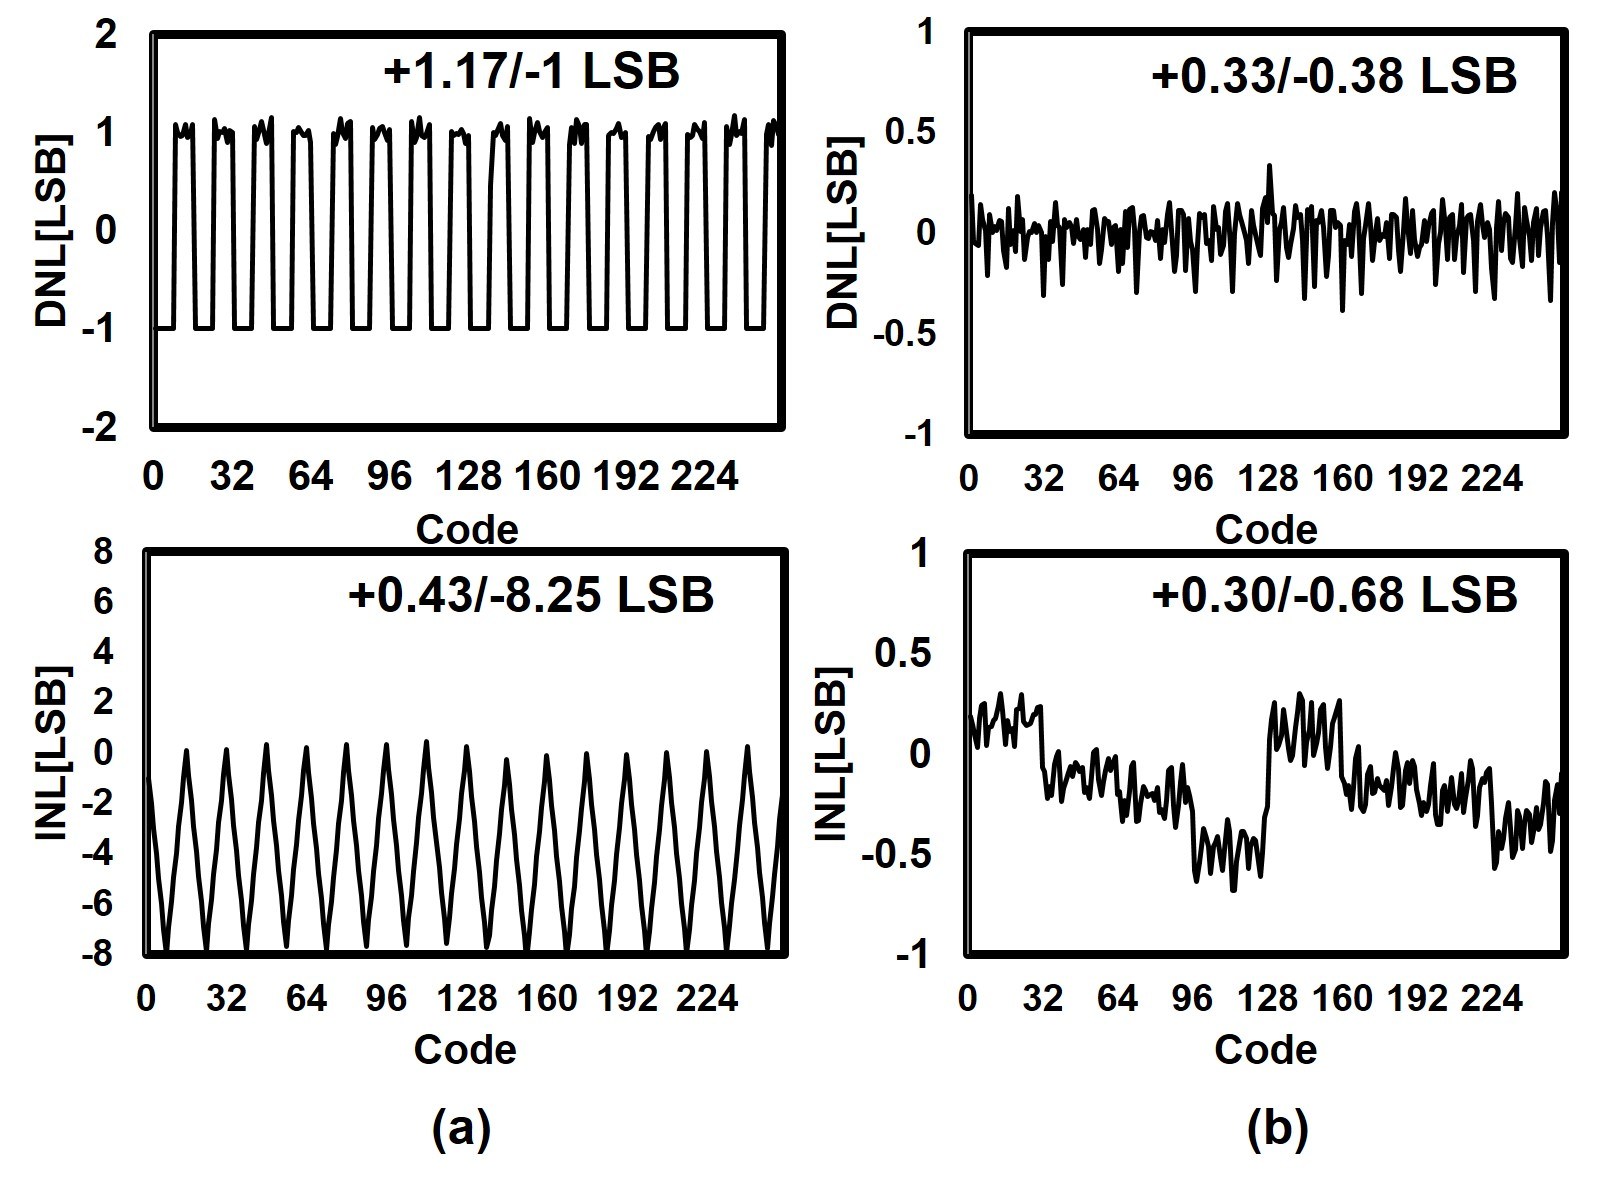
\includegraphics[width=0.9\textwidth]{figure/chap4/fig11.jpg}
  \caption{(a)DNL and INL before calibration at supply voltage of 0.5 V.
(b)DNL and INL after calibration at supply voltage of 0.5 V.}
  \label{fig-4-11}
\end{figure}

The proposed ADC prototype was designed and fabricated in a 1P7M 40nm standard CMOS process. Fig.\ref{fig-4-10} shows the microphotograph and layout of the chip. The core area is only 0.0153mm$^2$ and dummy layers are not removed since the effects can be removed by calibration.

Fig.\ref{fig-4-11} (a) and (b) show the DNL and INL at before and after calibration at a power supply of 0.5V, respectively. Foreground calibration has been done automatically with Matlab, under the same power supply. Before the calibration, a large number of miscodes were confirmed, resulting from C-DAC and VCS process mismatch. After the calibration, both DNL and INL are kept within 1 LSB and the effectiveness of calibration by internally generated reference is proved.

\begin{figure}
\centering
  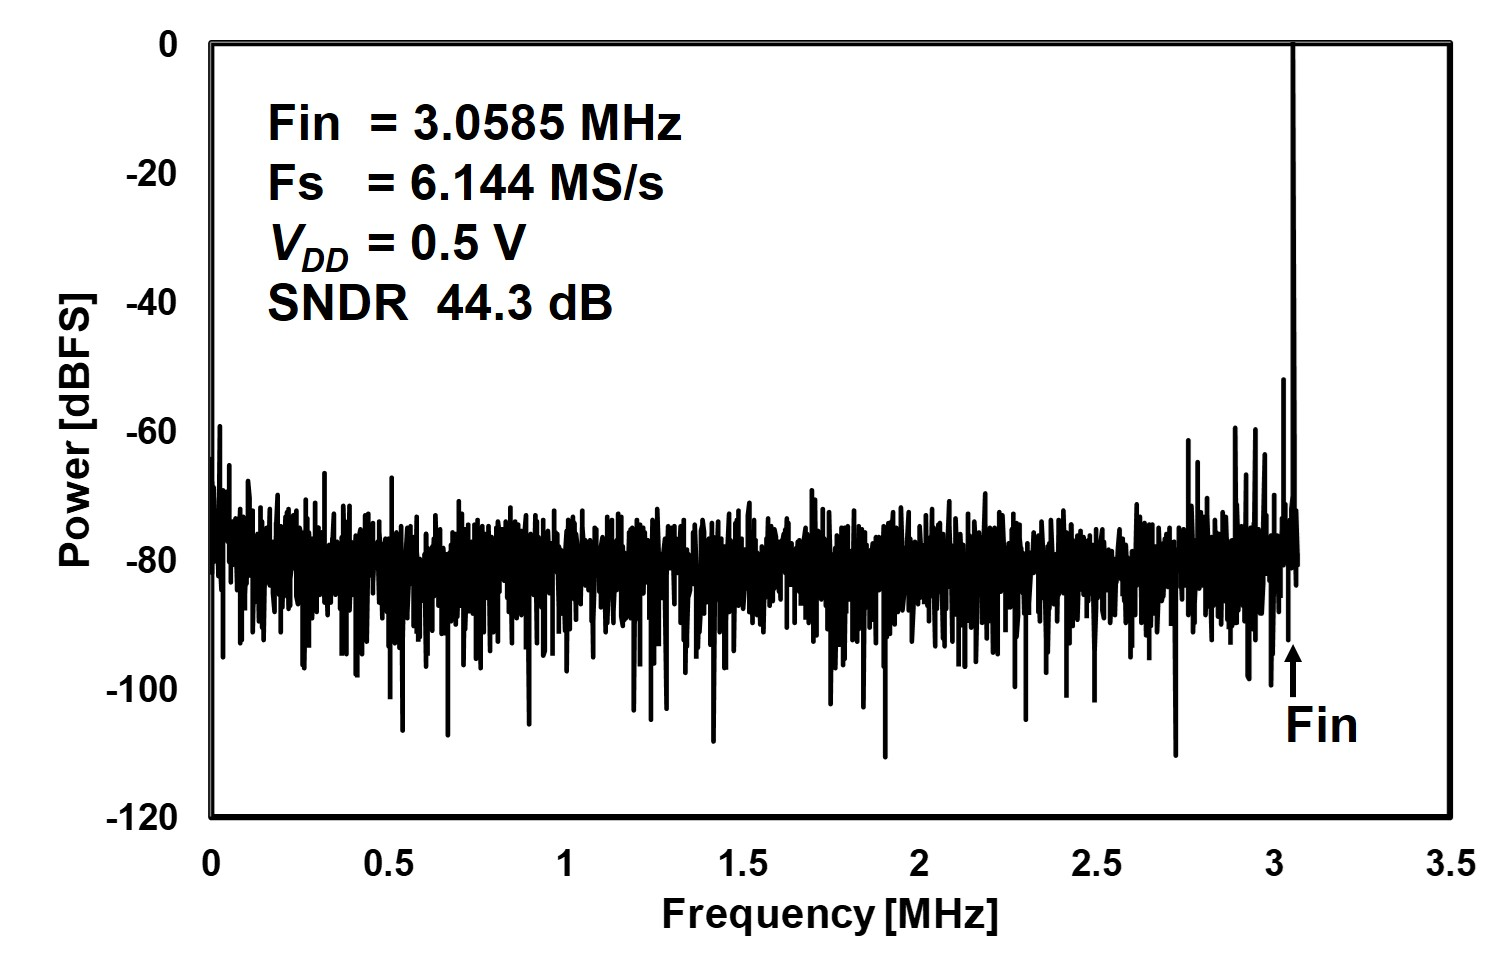
\includegraphics[width=0.9\textwidth]{figure/chap4/fig12.jpg}
  \caption{FFT spectrum at condition shown.}
  \label{fig-4-12}
\end{figure}
\begin{figure}
\centering
  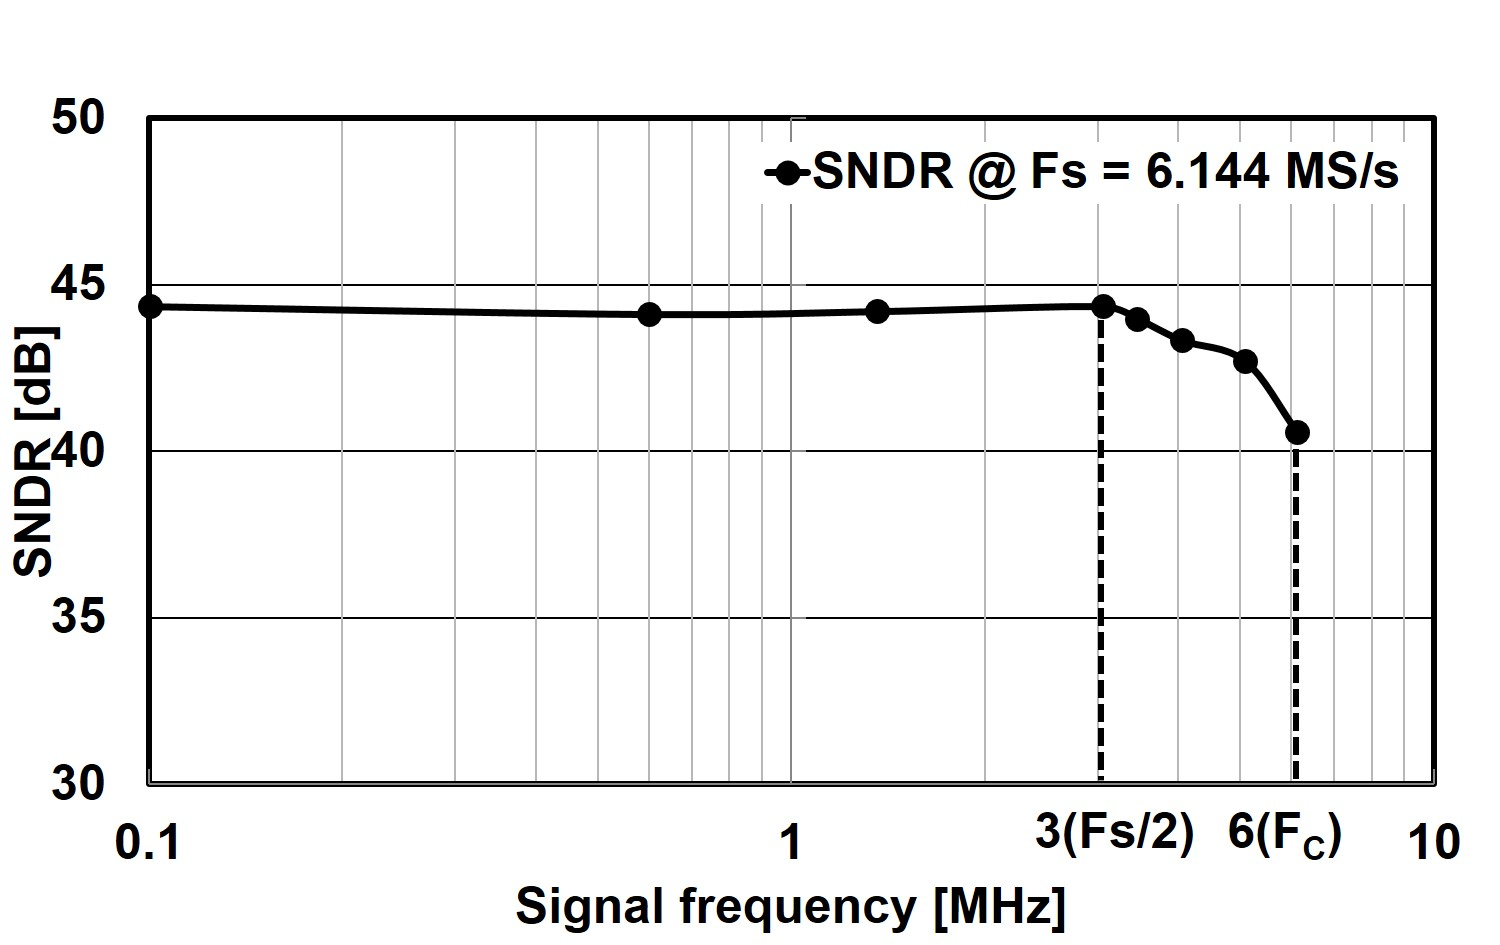
\includegraphics[width=0.9\textwidth]{figure/chap4/fig13.jpg}
  \caption{Input signal frequency versus SNDR measured at 0.5 V.}
  \label{fig-4-13}
\end{figure}


Fig. \ref{fig-4-12} shows the measured FFT spectrum with 6.144MS/s sampling frequency and Nyquist input frequency of 3.0585MHz. Fig. \ref{fig-4-13} represents the signal frequency vs. SNDR of the ADC at 0.5V. Flat frequency response was obtained between 100kHz and 3MHz (Nyquist frequency), and 3dB bandwidth is  6 MHz. The maximum ERBW was 50MHz measured at a power supply of 0.8V with a sampling frequency of 40.96MS/s.

\begin{figure}
\centering
  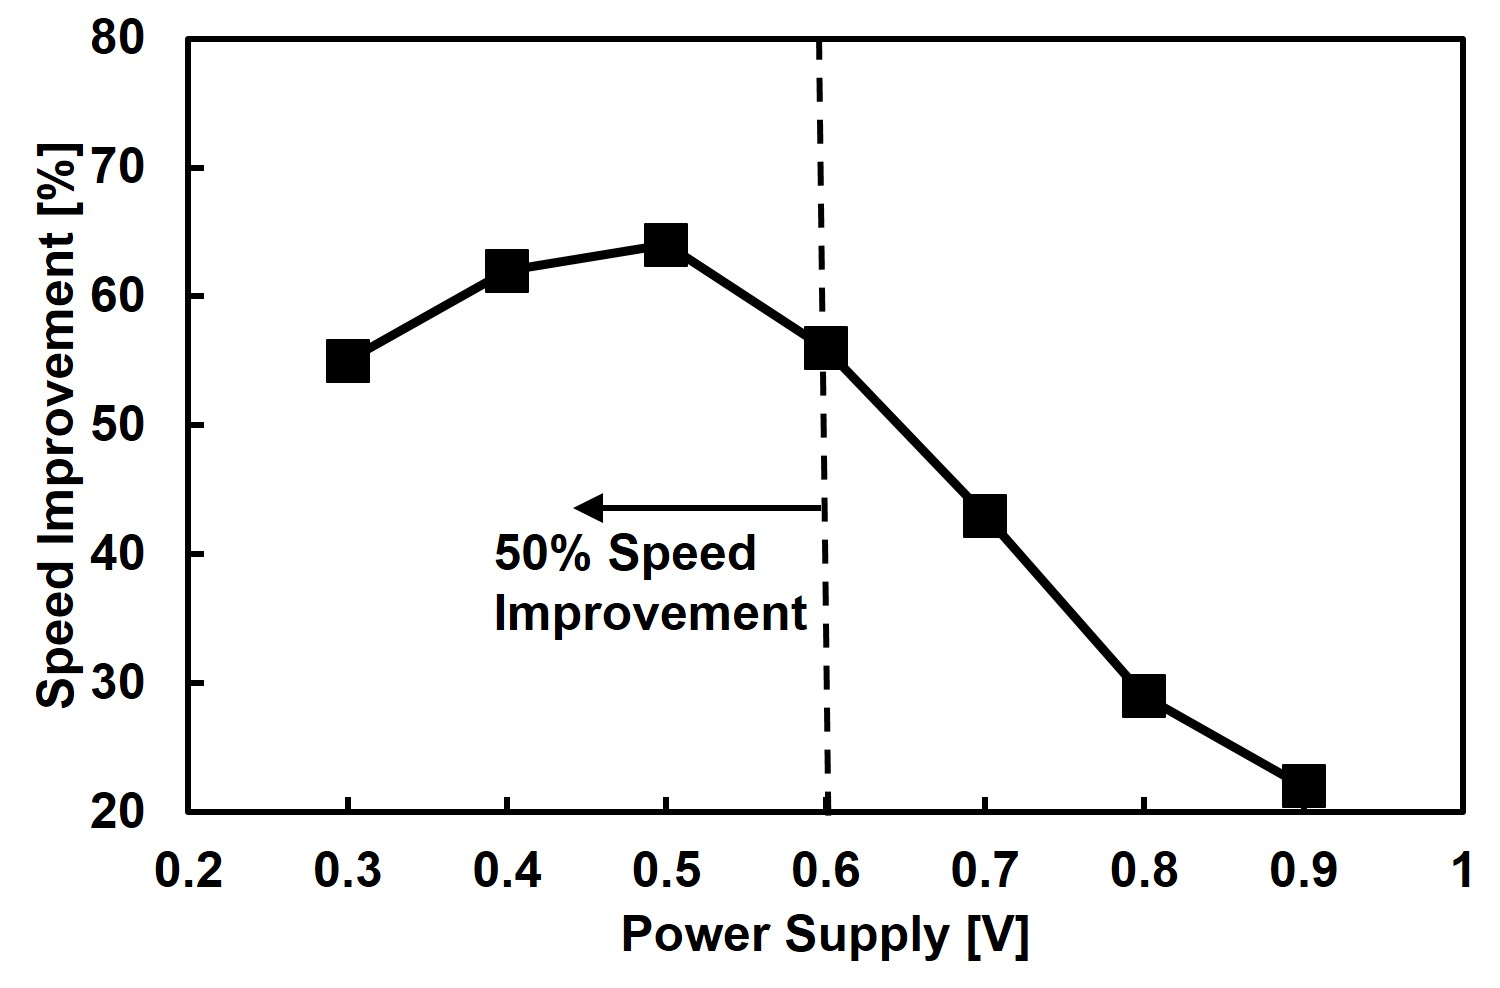
\includegraphics[width=0.9\textwidth]{figure/chap4/fig14.jpg}
  \caption{Power supply voltage versus speed improvement by 2-bit/step SAC operation.}
  \label{fig-4-14}
\end{figure}

Fig. \ref{fig-4-14} shows the power supply voltage vs. speed improvement comparing the 3dB cutoff frequency of 1-bit/step and 2-bit/step mode. By the proposed method, the ADC achieves maximum speed improvement of 60\% at 0.5V supply but falls beyond 30\% when the supply rises to 0.8V as DAC settling time shortens. However, at supply voltages below 0.4V, the speed improvement was smaller than expected. To maximize the SAR ADC speed, the asynchronous SAR logic delay should be set slightly longer than the DAC settling \cite{yoshioka-10b-50MS-SAR}. According to the post-layout simulation results, the minimum generatable delay of the asynchronous SAR logic was nearly twice as longer than the required DAC settling at such supply voltages. Such a delay generating circuit which can operate with a wide supply voltage range is challenging to design.

\begin{figure}
\centering
  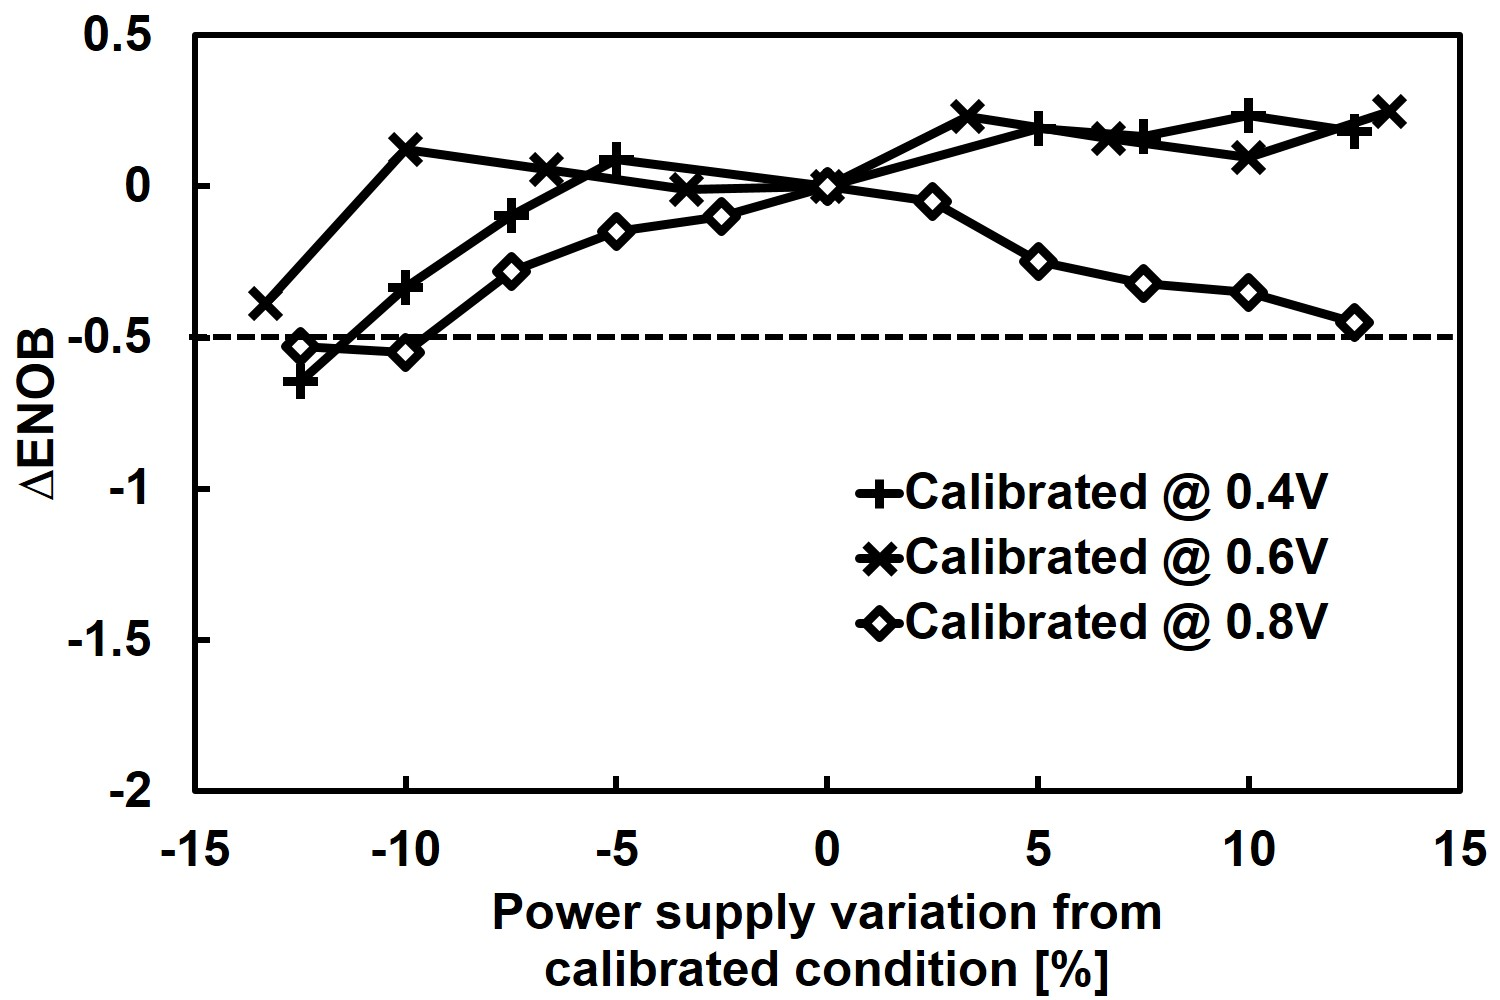
\includegraphics[width=0.9\textwidth]{figure/chap4/fig15.jpg}
  \caption{Power supply variation versus ENOB response in several calibrated supply voltages.}
  \label{fig-4-15}
\end{figure}
\begin{figure}
\centering
  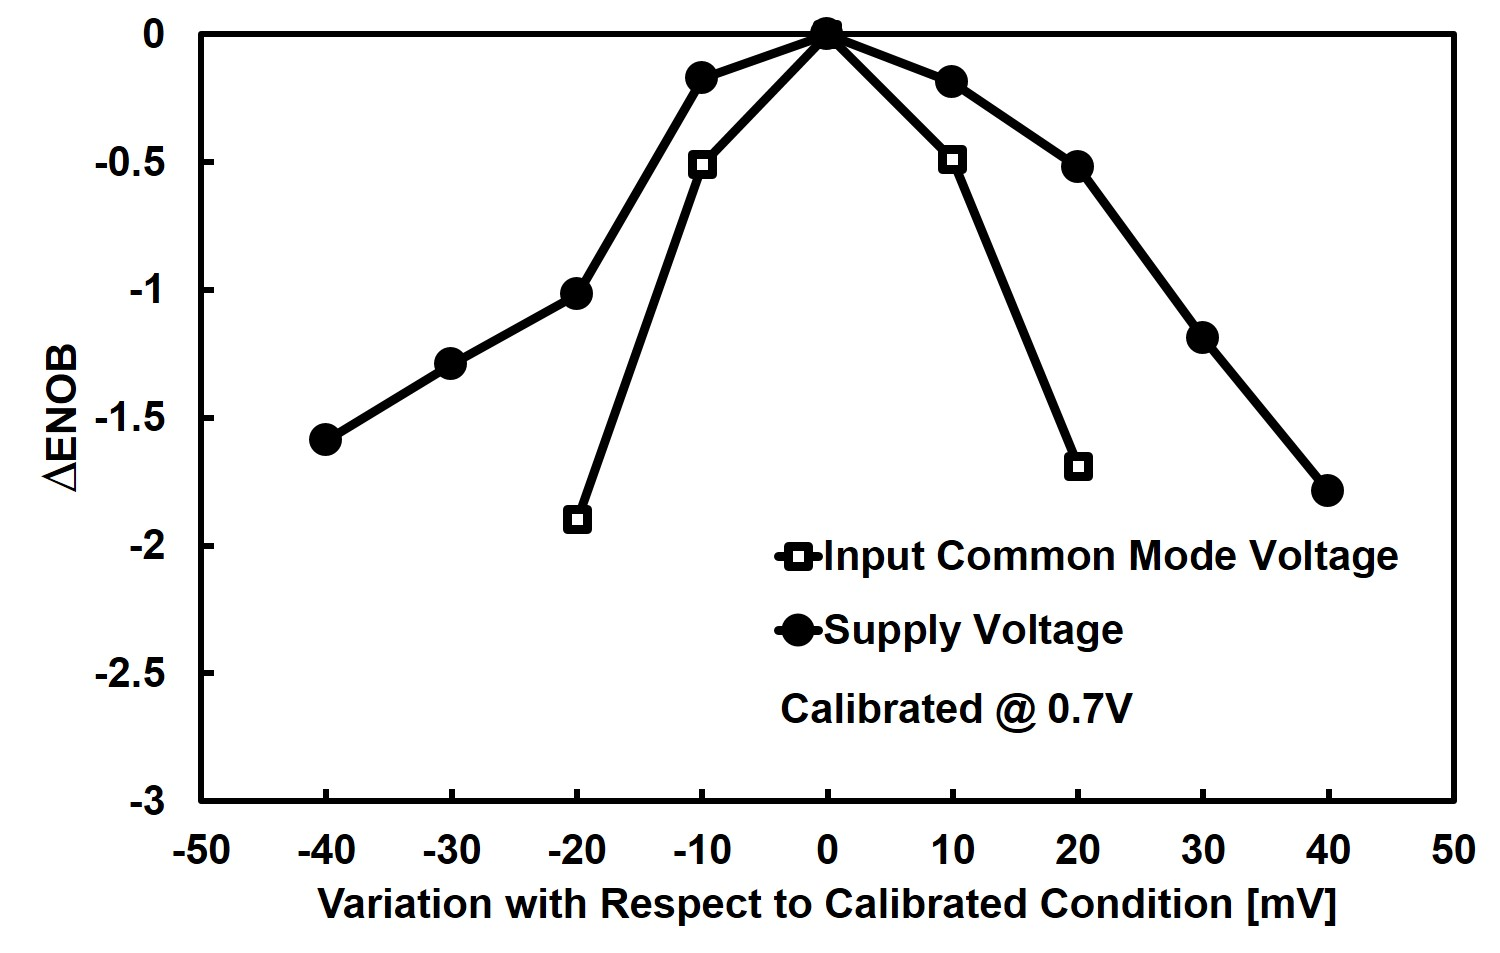
\includegraphics[width=0.9\textwidth]{figure/chap4/fig16.jpg}
  \caption{Effect of power supply variation with Vcm or VDD changed separately}
  \label{fig-4-16}
\end{figure}

Fig. \ref{fig-4-15} shows the SNDR dependence on the power supply voltage variation. The foreground calibration was done at multiple conditions noted and then power supply voltage was varied. $V_{CM}$ biased VCS has power supply noise immunity throughout the wide operating voltage. With a 10\% variation, the ENOB drop was only 0.5. In Fig. \ref{fig-4-15}, we assumed that the same power supply is used at the ADC input buffer and ADC itself so the power supply variation $\Delta V_{DD}$ is to be affected similarly. However, if the buffer and ADC are run on different supplies, the effect of variation will differ: only $V_{CM}$ varied or vice versa. The measurement result, in this case, is plotted in Fig.\ref{fig-4-16} and the ADC is tolerable of 10mV variance. To prevent resolution deteriorating due to low voltage operation, the calibration was done at 0.7V supply voltage. The measured ENOB degradation best matches when $C_{div}$/($C_{div}$+$C_p$)$-$0.5 was estimated as 0.25.

\begin{figure}
\centering
  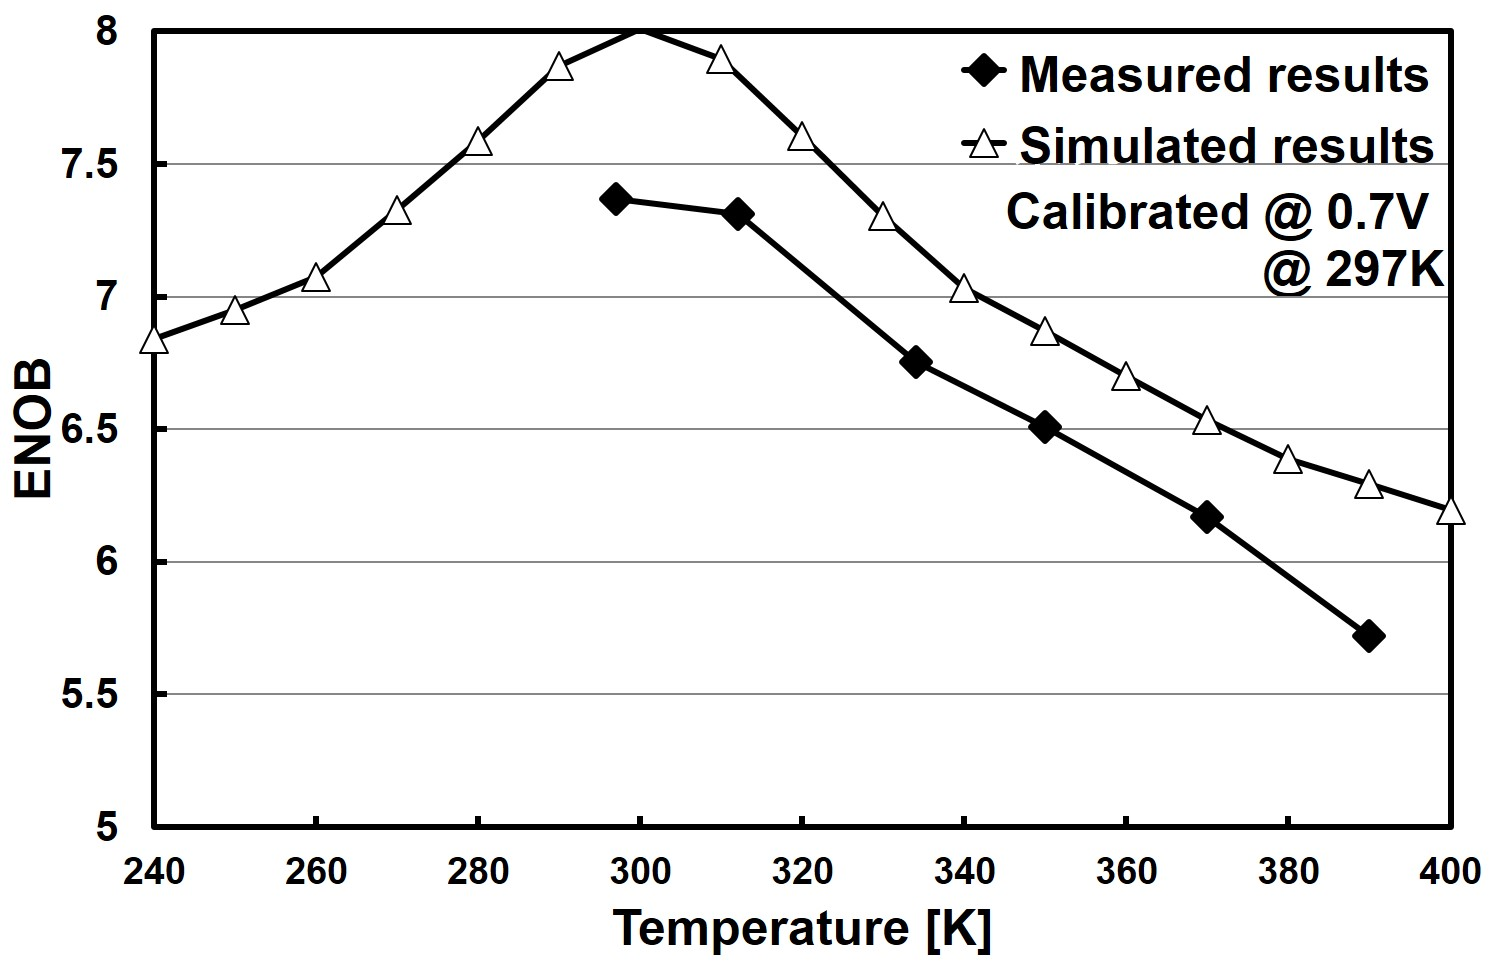
\includegraphics[width=0.9\textwidth]{figure/chap4/fig17.jpg}
  \caption{Simulated and measured temperature variation effects.}
  \label{fig-4-17}
\end{figure}

The temperature variation effect of this ADC is plotted in Fig.\ref{fig-4-17}. Calibration was done at 297K and the temperature was raised to measure the ENOB degradation. The degradation trend matches the simulation results. To compensate with temperature variation without periodic foreground calibrations, the additional biasing technique will be required as in \cite{nakajima-cal}. However, this technique has a very large power overhead and may consume more power than the ADC itself. Low-temperature measurements were not done because of lacked instruments but simulation results imply that 6.5bit can be achieved with 200K.

\begin{table}
    \centering
    \caption{ADC performance summary.}
    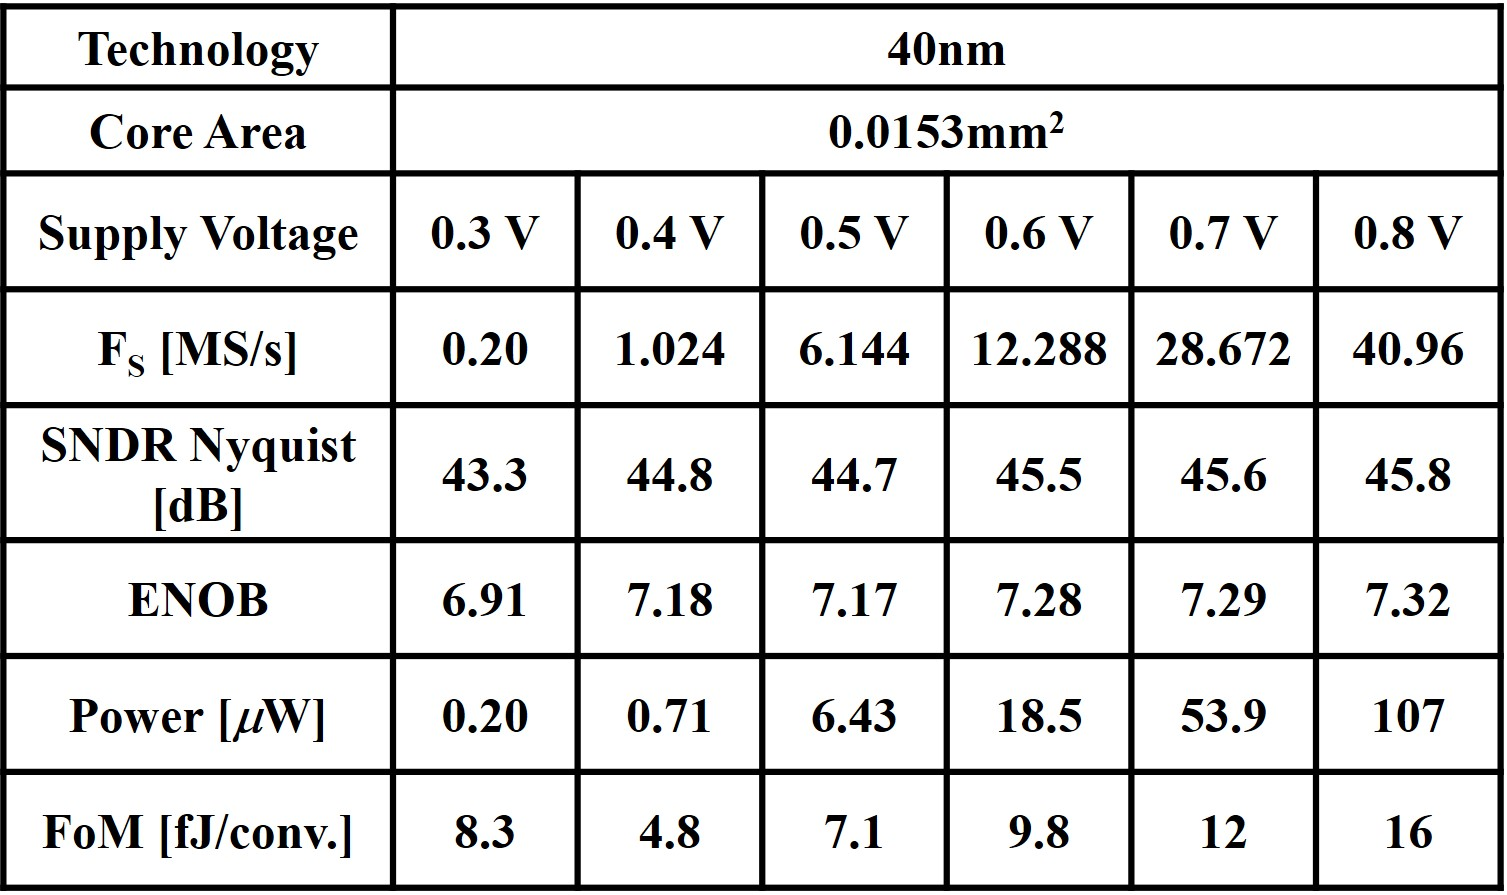
\includegraphics[width=1\textwidth]{figure/chap4/fig18.jpg}
    
    \label{tab:4-2}
\end{table}

\begin{figure}
\centering
  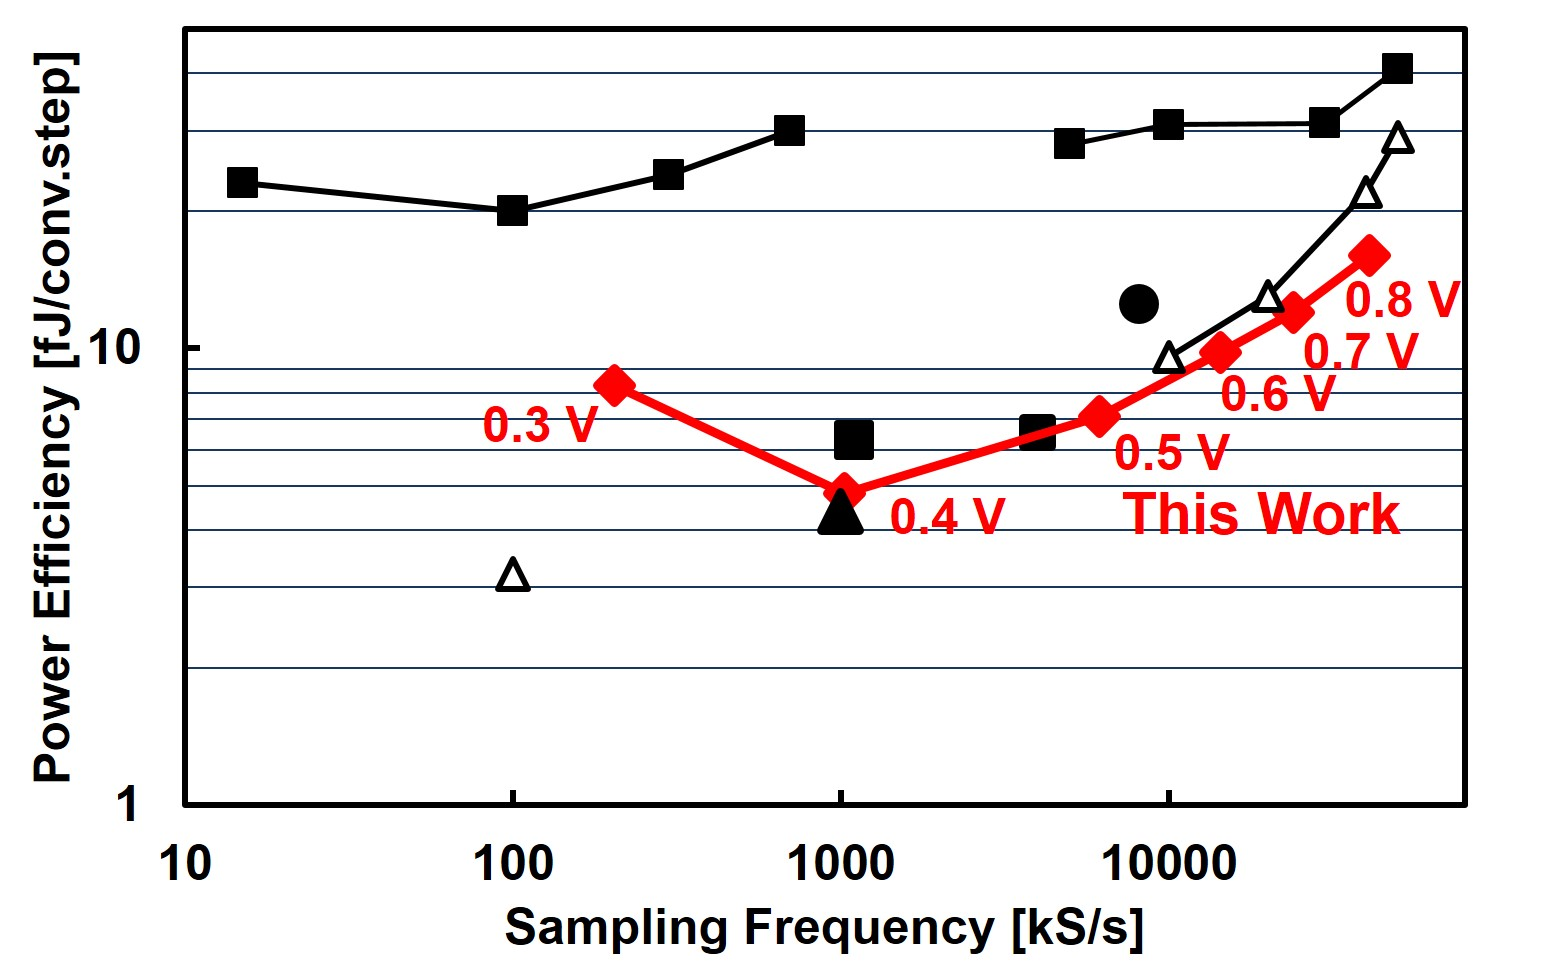
\includegraphics[width=1\textwidth]{figure/chap4/comparison.jpg}
  \caption{Comparison with low power state-of-art works.}
  \label{fig-4-18}
\end{figure}

The ADC performance of a single chip is summarized in TABLE \ref{tab:4-2} and performance comparison with low power state-of-art works is shown in Fig. \ref{fig-4-18}. Our ADC operates down to 0.3V while keeping an excellent FoM. The threshold configuring method by $V_{CM}$ bias current sources can be effective in such an extremely low voltage region as well. The achieved FoM throughout the operating supply voltage range of 0.3-0.8V is comparable with the other works which were designed for a dedicated specification. Moreover, the power efficiency is better than that of ADCs which operate in multiple voltages.

While our work was one of the pioneers seeking efficiencies with sub-0.5V operated SAR ADCs and when our paper was published, only a few SAR ADCs reported the operation yet \cite{tai20123}. Now, several 0.3V SAR ADC with extreme efficiencies (up to 1fJ/conv.) have been presented \cite{03VSAR} \cite{03VSAR2} \cite{03VSAR3}, showing that lowering the power supplies are one of the best ways to obtain top FoM with SAR ADCs.  

\section{Conclusions}

An extremely low-voltage operating high speed and low power SAR ADC was presented. Using wide-range threshold configuring comparators, a 2-bit/step operation was enabled with a small area and low power consumption. A comparator threshold configuring technique by $V_{CM}$ bias current sources was introduced. Compared with conventional threshold configuring techniques, the proposed method can generate large comparator offset with small power. Moreover, we proposed a novel design of the variable current source, with power supply noise immunity. The effect was confirmed by measurement and ADC had immunity against power supply variation of over 10\%. 

The prototype ADC achieved 6.1MS/s and 44.3dB SNDR with a power supply of 0.5V. 
At the supply of 0.4V, the ADC achieves a peak FoM of 4.8fJ/conv. and operates down to 0.3V. With the proposed techniques, the ADC achieved over 50\% speed improvement and achieved power efficiency competing with the state-of-the-art works.
